% =============================================================================
% Bachelor's Thesis -- Higher School of Economics
% Faculty of Computer Science
% Programme: Data Science and Business Analytics (01.03.02)
%
% Title: Community Detection with Graph Neural Networks via QUBO formulation
% =============================================================================

\documentclass[12pt,a4paper]{article}

% --- HSE Annex 7 formatting requirements ---
\usepackage[left=25mm, right=10mm, top=20mm, bottom=20mm]{geometry}

% Font: Times New Roman
\usepackage{mathptmx}
\usepackage[T1]{fontenc}
\usepackage[utf8]{inputenc}
\usepackage[english]{babel}


% Line spacing 1.5
\usepackage{setspace}
\onehalfspacing

% Paragraph formatting
\setlength{\parindent}{1.25cm}
\setlength{\parskip}{0pt}
\sloppy

% Page numbering
\usepackage{fancyhdr}
\pagestyle{plain}

% Math
\usepackage{amsmath, amssymb, amsthm}
\usepackage{mathtools}
\usepackage{algorithm}
\usepackage{algpseudocode}


% Figures and tables
\usepackage{graphicx}
\usepackage{float}
\usepackage{caption}
\captionsetup[figure]{labelsep=endash, name=Figure, labelfont=normalfont}
\captionsetup[table]{labelsep=endash, name=Table, labelfont=normalfont, justification=raggedright, singlelinecheck=false}
\usepackage{booktabs}
\usepackage{array}
\usepackage{multirow}

% Code listings
\usepackage{listings}
\usepackage{xcolor}
\lstdefinestyle{thesis_code}{
    basicstyle=\ttfamily\fontsize{10}{12}\selectfont,
    keywordstyle=\color{blue},
    commentstyle=\color{gray},
    stringstyle=\color{red!70!black},
    breaklines=true,
    showstringspaces=false,
    frame=single,
    numbers=left,
    numberstyle=\tiny\color{gray},
    aboveskip=10pt,
    belowskip=10pt,
}
\lstset{style=thesis_code}

% References [1], [2-3]
\usepackage[numbers,sort&compress]{natbib}
\bibliographystyle{unsrtnat}

\usepackage[hidelinks]{hyperref}

% Custom commands -- math notation
\newcommand{\B}{\mathbf{B}}
\newcommand{\Q}{\mathbf{Q}}
\newcommand{\xb}{\mathbf{x}}
\newcommand{\pb}{\mathbf{p}}
\newcommand{\Pb}{\mathbf{P}}
\newcommand{\Lcal}{\mathcal{L}}
\newcommand{\Ncal}{\mathcal{N}}
\newcommand{\svec}{\mathbf{s}}
\newcommand{\Cscr}{\mathcal{C}}
\newcommand{\yb}{\mathbf{y}}

% =============================================================================
\begin{document}

% =============================================================================
% Title page -- HSE FCS DSBA bachelor's thesis
% Following the official template (Sample_Title_List_ENG_DSBA)
% =============================================================================

\thispagestyle{empty}

\begin{center}
\vspace*{0pt}

National Research University Higher School of Economics

\vspace{4pt}

Faculty of Computer Science

\vspace{4pt}

Bachelor's Programme \emph{Data Science and Business Analytics}

\vspace{4pt}

01.03.02 Applied Mathematics and Information Science

\vspace{80pt}

{\Large\textbf{Community Detection with Graph Neural Networks via QUBO Formulation}}

\vspace{40pt}

{\large Bachelor's Thesis}

\end{center}

\vspace{60pt}

\begin{flushright}
\textit{Fulfilled by} \\[10pt]

\textbf{Rozinskiy Sergey Ivanovich} \\
\small (Student) \\[20pt]

\rule{6cm}{0.4pt} \\
\small (signature)
\end{flushright}

\vspace{40pt}

\begin{flushright}
\textit{Supervised by} \\[10pt]

\textbf{Ermakov Andrey Maksimovich} \\
\small Postgraduate Student, Faculty of Computer Science \\[20pt]

\rule{6cm}{0.4pt} \\
\small (signature)
\end{flushright}

\vfill

\begin{center}
Moscow, 2026
\end{center}

\newpage

\setcounter{page}{2}

% =============================================================================
% Abstract (200-350 words)
% =============================================================================

\section*{Abstract}
\addcontentsline{toc}{section}{Abstract}

Community detection is a fundamental problem in network science,
with applications in social network analysis, fraud detection, and
biological systems. The practical standard remains classical
heuristics such as Louvain~\cite{blondel2008louvain} and
Leiden~\cite{traag2019leiden}, although recent work has explored
formulating community detection as a Quadratic Unconstrained Binary
Optimization (QUBO) problem and solving it on specialized hardware
such as quantum annealers and Coherent Ising Machines. These
hardware-based approaches deliver promising results but remain
inaccessible to most practitioners.

This thesis develops a software-based alternative to hardware QUBO
solvers for community detection. The starting point is the QIGNN
framework~\cite{qignn2026}~--~an unsupervised graph neural network
originally validated on two-class (single-bit-per-vertex) combinatorial problems such as
MaxCut and Maximum Independent Set. The QIGNN paradigm is extended
to the multi-class setting of community detection, combining the
QUBO formulations of modularity maximization due to Wang et
al.~\cite{wang2024quantum} with the neural-relaxation approach of
Schuetz et al.~\cite{schuetz2022combinatorial}.

The QIGNN architecture is adapted to the multi-class community
assignment task through a softmax output layer over $k$ classes and
the linearization of the QUBO problem required for handling one-hot
encoded variables. An orthogonality regularization adapted
from~\cite{bianchi2020spectral} is integrated to control the
trivial-collapse failure mode of the multi-class loss landscape, and
its behaviour is analyzed across graph structures of varying
balance. A memory-efficient training procedure is developed that
computes the QUBO loss directly from the modularity matrix and the
probability matrix, without materializing the full QUBO matrix. This
reduces the memory footprint of the multi-class loss by a factor of
$k^{2}$ in the number of communities, making training feasible on
graphs that would otherwise be out of reach.

The bipartition formulation of the proposed method converges
deterministically on the binary benchmarks considered and
reaches normalized mutual information at or above Louvain's on
the majority of them. Where the direct multi-class formulation
runs into difficulties, a hierarchical extension is proposed that
recursively applies the bipartition formulation. The hierarchical
algorithm exposes two operating modes with different trade-offs:
the fully automatic modularity-gain mode matches Louvain in
modularity within $0.02$ on every benchmark tested (up to $42$
ground-truth communities) and exceeds Louvain in NMI on four of
them; the target-$k$ mode (which requires the number of
communities as input) trades a modularity gap on imbalanced
graphs for higher NMI, matching or exceeding Louvain on ten of
thirteen benchmarks. The algorithm inherits the empirical
determinism of the bipartition formulation across both modes.
The applicability regime of each formulation is analyzed in
terms of problem size, community balance, and number of classes.

Together, these results establish QIGNN-based community detection
as a viable commodity-hardware alternative to hardware QUBO
solvers, competitive with classical heuristics across both binary
and multi-class settings.

\bigskip

\textbf{Keywords:} community detection, graph neural networks, QUBO,
modularity, combinatorial optimization, unsupervised learning.

\newpage
\newpage

\tableofcontents
\newpage

% =============================================================================
% Chapter 1: Introduction (3-4 pages)
% =============================================================================

\section{Introduction}
\label{sec:introduction}

\subsection{Motivation}
\label{sec:motivation}

Many graphs of interest exhibit community structure: their vertices
form groups that are more densely connected internally than to the
rest of the graph. Examples include friendship circles in social
networks, functional protein complexes in biological systems, and
clusters of behaviorally similar customers in financial networks.
Recovering this structure from the graph alone, without external
labels, is the problem of \emph{community
detection}~\cite{fortunato2010community}, with applications across
network science and, more recently, in anti-fraud
analytics~\cite{wang2024quantum}.

The dominant practical approach is to maximize Newman's
modularity~\cite{newman2006modularity} through local greedy search,
as in the Louvain~\cite{blondel2008louvain} and
Leiden~\cite{traag2019leiden} algorithms. These methods are fast and
deliver high-quality partitions on graphs of millions of vertices.
However, they are local heuristics: they do not in general find the
global modularity optimum, and they suffer from the \emph{resolution
limit}~\cite{fortunato2007resolution}, which prevents them from
detecting small communities embedded in larger graphs. These
limitations motivate the search for alternative approaches.

One alternative formulates modularity maximization as a Quadratic
Unconstrained Binary Optimization (QUBO)
problem~\cite{lucas2014ising}. The partition is then a vector of
binary variables, and modularity is a quadratic form over those
variables. The problem itself remains NP-hard, but the QUBO
formulation opens it to a different class of solvers: classical
local search~\cite{ushijima2017graph}, quantum
annealing~\cite{negre2020detecting}, and Coherent Ising
Machines~\cite{wang2024quantum}. Wang et
al.~\cite{wang2024quantum} recently demonstrated this last approach
on real banking data, but their method depends on specialized analog
hardware that is not widely available.

A different line of work, due to Schuetz et
al.~\cite{schuetz2022combinatorial}, replaces the dedicated hardware
with an unsupervised graph neural network. Their Physics-Inspired
GNN (PI-GNN) parameterizes the binary assignment vector through a
continuous relaxation and trains the GNN to minimize the relaxed
QUBO loss on a single GPU, without any labeled data. The QIGNN
framework~\cite{qignn2026} extends PI-GNN with iterative refinement:
the prediction of one training epoch is concatenated with the input
features of the next, allowing the network to revisit and improve
its earlier output. Both PI-GNN and QIGNN have so far been validated
on two-class (single-bit-per-vertex) combinatorial problems --- MaxCut and Maximum
Independent Set --- where each variable is a single binary
indicator.

The community detection problem reduces to a single-bit-per-vertex
formulation only in the special case of two communities. With $k > 2$ communities each vertex must
be assigned a one-hot vector of length $k$, the QUBO matrix grows
from $n \times n$ to $nk \times nk$, and the one-hot constraint
needs to be enforced through a penalty term in the loss. Whether
the QIGNN approach extends cleanly to this setting is the question
this thesis sets out to answer. The investigation produces both an
extension of the QIGNN framework to the multi-class case and, where
the multi-class formulation runs into difficulties, a hierarchical
algorithm that recovers competitive performance by recursively
applying the more reliable bipartition formulation.


\subsection{Problem statement}
\label{sec:problem_statement}

Let $G = (V, E)$ be an undirected graph with $|V| = n$ vertices and
$|E| = m$ edges. A \emph{community structure} on $G$ is a partition
of the vertex set into $k$ disjoint, non-empty subsets, encoded as
a function $C: V \to \{1, \ldots, k\}$ that assigns each vertex a
community label. The community detection problem asks for the
partition that best reflects the underlying structure of the graph,
where ``best'' is measured by a quality function on partitions.

Newman's modularity~\cite{newman2006modularity} is the quality
function adopted throughout this thesis. It is defined as
\begin{equation}
    M(C) = \frac{1}{2m} \sum_{v, w \in V}
    \left( A_{vw} - \frac{k_v k_w}{2m} \right)
    \delta(C_v, C_w),
    \label{eq:modularity_intro}
\end{equation}
where $A_{vw}$ is the adjacency matrix entry between vertices $v$
and $w$, $k_v = \sum_w A_{vw}$ is the degree of vertex $v$, and
$\delta$ is the Kronecker delta. The optimization problem is then
$C^* = \arg\max_{C} M(C)$.

Modularity maximization is NP-hard~\cite{brandes2008modularity}, so
exact solution is infeasible at any practical scale and approximate
methods are required. This thesis assumes that the number of
communities $k$ is given as part of the input. Determining $k$
automatically is its own line of research, and fixing it lets the
focus stay on the optimization itself.


\subsection{Approach overview}
\label{sec:approach_overview}

The approach combines a QUBO formulation of the modularity objective
with an unsupervised graph neural network as the solver. Given a
graph $G$ and a target number of communities $k$, the procedure has
three steps: (i) construct a QUBO matrix $\Q$ that encodes the
modularity objective; (ii) train a GNN whose output, after softmax
normalization, parameterizes a relaxed solution $\Pb(\theta) \in
[0,1]^{n \times k}$; (iii) recover a discrete partition by taking
$\arg\max$ along the community dimension of $\Pb$. The GNN is
trained from scratch on the input graph by minimizing the relaxed
QUBO loss $\Lcal(\theta) = \pb_{\mathrm{flat}}^T \, \Q \,
\pb_{\mathrm{flat}}$. No labeled data is used.

For the QUBO construction the formulations of Wang et
al.~\cite{wang2024quantum} are used. The bipartition formulation
($k=2$) encodes community membership through a single binary
variable per vertex and reduces to the quadratic form $\xb^T (-\B)
\xb$, where $\B$ is the modularity matrix. The multi-class
formulation ($k > 2$) introduces $nk$ binary variables under a
one-hot encoding constraint, which is enforced softly through a
quadratic penalty term. Both formulations are implemented in this
work.

For the neural solver the QIGNN framework~\cite{qignn2026} is used
as the starting point. QIGNN combines GraphSAGE convolutional
blocks with iterative refinement of the previous epoch's prediction.
The architecture is adapted to multi-class output by replacing the
sigmoid head with a softmax layer over $k$ classes. To make the
multi-class loss tractable on graphs of practical size, a
memory-efficient training procedure is developed that computes the
loss directly from the modularity matrix and the probability matrix
without ever materializing the full $nk \times nk$ QUBO matrix.

The multi-class loss has a wide local attractor at the trivial
all-in-one assignment, where every vertex is placed into the same
community. An orthogonality regularization adapted from
MinCutPool~\cite{bianchi2020spectral} is integrated to discourage
this collapse by penalizing overlap between community columns. Its
behavior is evaluated empirically on graphs with both balanced and
imbalanced community structures.

Training uses the Adam optimizer with a time-dependent annealing
penalty that pushes the relaxed solution toward the corners of the
hypercube as training progresses. A schematic of the architecture
and training loop is given in Section~\ref{sec:methodology}.


\subsection{Scientific novelty}
\label{sec:novelty}

The scientific novelty of this thesis is summarized in the
following points.

\begin{enumerate}
    \item \textbf{A hierarchical decomposition algorithm for
    multi-class community detection.} A new algorithm is proposed
    that recursively applies the stable bipartition QUBO
    formulation through QIGNN to recover community structure for
    arbitrary $k$, using modularity gain as the natural stopping
    criterion. To the best of the author's knowledge, this is the
    first work to combine QUBO-based neural solvers with
    hierarchical graph decomposition for community detection. The
    hierarchical method, in its automatic modularity-gain mode,
    matches Louvain in modularity within $0.02$ on every benchmark
    in the study (including graphs with up to forty-two
    ground-truth communities) and strictly exceeds Louvain in
    normalized mutual information on four of them. An optional
    target-$k$ mode that takes the ground-truth $k$ as input
    trades a modularity gap on imbalanced graphs for higher NMI,
    matching or exceeding Louvain on ten of thirteen benchmarks.
    The modularity-gain criterion automatically discovers the
    number of communities, recovering Louvain's choice of $k$
    on graphs where Louvain's heuristic is itself reliable.

    \item \textbf{Extension of the QIGNN framework to multi-class
    community detection.} The QIGNN
    framework~\cite{qignn2026} and its predecessor
    PI-GNN~\cite{schuetz2022combinatorial} have so far been
    validated only on two-class problems such as MaxCut and Maximum
    Independent Set. To the best of the author's knowledge, this
    thesis is the first to apply the QIGNN paradigm to community
    detection with arbitrary $k$. The extension involves a softmax
    output layer over $k$ classes and the linearization of one-hot
    encoded QUBO variables.

    \item \textbf{Empirical demonstration that the bipartition
    formulation of QIGNN matches or exceeds Louvain in agreement
    with ground-truth community structure.} On diverse binary
    community detection benchmarks the unsupervised QIGNN-based
    solver reaches normalized mutual information at or above
    Louvain's. This result has not, to the author's knowledge,
    been previously reported.

    \item \textbf{Memory-efficient training procedure for the
    multi-class QUBO loss.} The proposed implementation computes
    the QUBO loss directly from the modularity matrix and the
    probability matrix, without materializing the full QUBO
    matrix. This reduces memory complexity from quadratic to
    linear in the linearized problem size and makes training
    feasible on graphs that the original PI-GNN and QIGNN
    implementations cannot handle.

    \item \textbf{Analysis of orthogonality regularization in the
    QUBO setting.} The orthogonality regularization originates in
    the supervised MinCutPool method~\cite{bianchi2020spectral}
    (and is also used by DMoN~\cite{tsitsulin2020graph}); its
    behavior in the unsupervised QUBO setting has not previously
    been studied. A systematic empirical comparison across diverse
    graph structures is provided, identifying when the
    regularization helps and when its built-in balance prior
    actively harms performance on imbalanced graphs.
\end{enumerate}


\newpage
\newpage

% =============================================================================
% Chapter 2: Related Work (4-5 pages)
% =============================================================================

\section{Related Work}
\label{sec:related_work}

This chapter demonstrates the contribution of the thesis within the framework of four
areas of previous work: the formulation of community detection as a
quality-function optimization problem, QUBO-based approaches and
their hardware solvers, neural network methods for community
detection, and the unsupervised QUBO-via-GNN paradigm that the
thesis builds on. The chapter closes with a brief discussion of the
trivial collapse phenomenon, which motivates the regularization
analysis in later sections.

% -----------------------------------------------------------------------------
\subsection{Community detection problem}
\label{sec:rw_problem}

\subsubsection{Modularity and its limitations}
\label{sec:rw_modularity}

Community detection has been studied for over two decades; surveys
such as Fortunato~\cite{fortunato2010community} cover the main
threads. The dominant quality function is Newman's
modularity~\cite{newman2006modularity}, defined in
equation~\eqref{eq:modularity_intro}. Modularity compares the
observed edge density inside each community to the density expected
in a random graph with the same degree sequence, and high modularity
is interpreted as evidence of community structure.

Despite its widespread use, modularity has known issues. The
\emph{resolution limit} of Fortunato and
Barth\'elemy~\cite{fortunato2007resolution} shows that maximizing
modularity in large graphs systematically merges small communities
into larger ones, even when the small communities are well defined.
Modularity is also degenerate in the sense of Good et
al.~\cite{good2010performance}: many partitions of a real-world
graph achieve modularity close to the maximum, so the optimum is
neither unique nor robust. Alternative quality functions such as
normalized cut and conductance~\cite{shi2000normalized} avoid some
of these issues at the cost of different trade-offs. This thesis
keeps modularity as the optimization target, both because it is the
objective in the QUBO formulations of Wang et
al.~\cite{wang2024quantum} that the thesis adopts, and because
modularity remains the standard against which community detection
methods are typically compared.

\subsubsection{Classical algorithms}
\label{sec:rw_classical}

The Louvain algorithm of Blondel et al.~\cite{blondel2008louvain}
optimizes modularity through a two-phase greedy procedure. In the
first phase, vertices are repeatedly moved between communities to
greedily increase modularity; in the second phase, the resulting
communities are aggregated into super-vertices and the process is
repeated on the smaller graph. The Leiden algorithm of Traag et
al.~\cite{traag2019leiden} refines Louvain by adding a vertex-level
refinement step that guarantees connected communities and avoids
some pathological cases of Louvain. Both algorithms run in nearly
linear time on sparse graphs and are the de facto baselines for
modularity-based community detection.

Other classical approaches include spectral methods, which relax the
discrete partition problem to a continuous eigenvector problem on
the graph Laplacian or the modularity
matrix~\cite{newman2013spectral, shi2000normalized}, and
information-theoretic methods such as
Infomap~\cite{rosvall2008infomap}, which finds communities by
minimizing the description length of a random walk on the graph.
Stochastic block models~\cite{karrer2011stochastic} take a generative
view of the problem and recover communities through statistical
inference. The thesis uses Louvain as the primary baseline
because it shares the modularity objective with the proposed
method, making the comparison meaningful; Leiden is reported
alongside Louvain in the dataset-level baseline table
(Section~\ref{sec:exp_baselines_metrics}) as a sanity check and
behaves within a few thousandths of Louvain on every benchmark.

% -----------------------------------------------------------------------------
\subsection{QUBO formulations and hardware solvers}
\label{sec:rw_qubo}

\subsubsection{QUBO and Ising}
\label{sec:rw_lucas}

A Quadratic Unconstrained Binary Optimization (QUBO) problem
minimizes a quadratic form $\xb^T \Q \xb$ over binary vectors $\xb
\in \{0,1\}^N$. The QUBO problem is equivalent to the Ising spin
model under the change of variables $s_i = 2 x_i - 1$, mapping $\xb
\in \{0,1\}^N$ to $\mathbf{s} \in \{-1, +1\}^N$. This equivalence is
useful because the Ising model has a long history in physics and
because both quantum and analog hardware solvers are typically built
in the Ising form.

Lucas~\cite{lucas2014ising} provides the standard reference catalog
of NP-hard problems formulated as Ising/QUBO problems, including
maximum cut, graph coloring, traveling salesman, and others. This
catalog enables a single hardware solver to address a wide range of
combinatorial problems by translating each problem into the
hardware's native form.

\subsubsection{QUBO for community detection}
\label{sec:rw_qubo_cd}

The use of QUBO for community detection traces back to the
graph-partitioning formulation of Ushijima-Mwesigwa et
al.~\cite{ushijima2017graph}, who solved a balanced 2-way partition
problem on the D-Wave quantum annealer. Negre et
al.~\cite{negre2020detecting} extended the approach to multi-way
community detection by introducing one-hot encoded community
indicators with a soft constraint penalty, which is the
multi-class formulation later adopted by Wang et
al.~\cite{wang2024quantum}.

The most direct precursor of this thesis is the work of Wang et
al.~\cite{wang2024quantum}, which formulates modularity maximization
as both a bipartition QUBO (formula~6 in their paper, used here as
the basis of Section~\ref{sec:method_qubo_k2}) and a multi-class
QUBO (formula~5, used in Section~\ref{sec:method_qubo_multi}). They
solve the resulting QUBO instances on a Coherent Ising Machine
(CIM) and apply the method to a real banking fraud detection
dataset. Their results demonstrate that QUBO-based community
detection can match or exceed classical heuristics in some settings,
but the underlying solver depends entirely on specialized analog
hardware.

\subsubsection{Hardware solvers and their limitations}
\label{sec:rw_hardware}

Hardware QUBO solvers fall into two main families. Quantum annealers
such as the D-Wave systems implement the Ising model on a network
of physical qubits and find low-energy states through quantum
tunneling. Coherent Ising Machines, used by Wang et
al.~\cite{wang2024quantum}, implement the Ising model through
optical parametric oscillators and rely on synchronization dynamics
rather than quantum tunneling. Both families share two practical
limitations. First, the available system size is bounded by the
hardware's number of qubits or oscillators, with current systems
supporting at most a few thousand variables. For multi-class
community detection this corresponds to graphs with at most a few
hundred vertices when $k$ is moderate. Second, both families require
specialized hardware that is not widely accessible.

These limitations motivate the search for software-based QUBO
solvers that run on commodity hardware while preserving the global
nature of the QUBO formulation. The unsupervised neural approach
discussed in Section~\ref{sec:rw_unsupervised} is one such direction.

% -----------------------------------------------------------------------------
\subsection{GNN-based community detection}
\label{sec:rw_gnn_cd}

\subsubsection{Graph neural networks}
\label{sec:rw_gnn_arch}

Graph neural networks (GNNs) operate on graph-structured data by
iteratively updating vertex embeddings based on the embeddings of
neighboring vertices. The graph convolutional network (GCN) of Kipf
and Welling~\cite{kipf2017semi} popularized this class of models;
GraphSAGE~\cite{hamilton2017inductive} introduced sampled and
concatenation-based aggregation; the graph attention network
(GAT)~\cite{velickovic2018graph} added learned attention weights
between neighbors; and GIN~\cite{xu2019gin} provided theoretical
guarantees on representational power. The methodology in this
thesis builds on a GraphSAGE backbone, following the choice made by
the QIGNN framework discussed in Section~\ref{sec:rw_qignn}.

\subsubsection{Supervised approaches: DMoN}
\label{sec:rw_dmon}

Tsitsulin et al.~\cite{tsitsulin2020graph} proposed the
Differentiable Modularity Optimization Network (DMoN), which uses
a GNN to map vertex features to soft community assignments and
trains the GNN end-to-end by maximizing a differentiable surrogate
of modularity. DMoN is supervised in the sense that it requires
node features (typically derived from labeled data) but is
unsupervised in its training signal: only the modularity-based loss
is used, with no community labels.

DMoN includes an orthogonality regularization that penalizes
overlap between community assignments. The specific orthogonality
formula
$\bigl\| \Pb^T \Pb / \| \Pb^T \Pb \|_F - I_k / \sqrt{k} \bigr\|_F^2$
adopted in Section~\ref{sec:method_ortho} of this thesis is the
form introduced by MinCutPool~\cite{bianchi2020spectral} and also
used by DMoN; both papers report it as effective against
degenerate cluster assignments. This thesis applies it in the
rather different setting of an unsupervised QUBO loss.

A related supervised method is MinCutPool by Bianchi et
al.~\cite{bianchi2020spectral}, which uses a normalized minimum
cut as the training signal and includes a similar orthogonality
regularization. Both methods rely on supervised features and are
designed for graph-level pooling rather than full community
detection on a single graph.

% -----------------------------------------------------------------------------
\subsection{Unsupervised neural QUBO solvers}
\label{sec:rw_unsupervised}

\subsubsection{PI-GNN}
\label{sec:rw_pignn}

The Physics-Inspired GNN (PI-GNN) of Schuetz et
al.~\cite{schuetz2022combinatorial} is the starting point for the
line of work this thesis extends. Given a QUBO instance defined by
a matrix $\Q$, PI-GNN trains a GNN whose output is a vector of
relaxed assignments $\pb \in [0,1]^N$, and the GNN is trained on a
single graph by minimizing the relaxed QUBO loss $\pb^T \Q \pb$,
without any labeled data. After training, the relaxed solution is
rounded to a binary vector. The approach is validated on Maximum
Independent Set and MaxCut benchmarks, where PI-GNN matches or
exceeds classical heuristics on a number of instances while running
on a single GPU.

The key insight of Schuetz et al.\ is that the GNN provides an
implicit regularization through the graph structure: vertices that
are close in the graph receive similar embeddings, which translates
to similar relaxed assignments. This makes the optimization easier
than direct gradient descent on $\pb$ in $\mathbb{R}^N$, where no
such structure is exploited.

\subsubsection{QIGNN}
\label{sec:rw_qignn}

The QIGNN framework~\cite{qignn2026} extends PI-GNN with iterative
refinement. At each training epoch, the network's previous-epoch
output is concatenated with its static input features, so that the
GNN can revisit and improve its earlier prediction. The
architecture itself uses GraphSAGE blocks with two parallel
aggregations (mean and max-pool) combined through a residual
connection, giving a richer neighborhood representation than a
single-aggregator GraphSAGE block. The framework is validated on
the same MaxCut and MIS benchmarks as PI-GNN and reports improved
stability and final solution quality.

QIGNN is the architectural starting point of this thesis. The
existing validation of QIGNN is restricted to two-class
combinatorial problems, where each variable is a single binary
indicator; the present thesis is, to the best of the author's
knowledge, the first work to apply the QIGNN paradigm to a
multi-class problem.

\subsubsection{Limits of neural QUBO solvers}
\label{sec:rw_critique}

The unsupervised neural QUBO solver paradigm has been challenged.
Angelini and Ricci-Tersenghi~\cite{angelini2023modern} argue that
on Maximum Independent Set the original PI-GNN is outperformed by a
simple greedy degree-based heuristic, and that the apparent
strength of PI-GNN in the original paper is partly due to the choice
of benchmark instances. Their critique does not invalidate the
general approach, but it does highlight the importance of careful
empirical evaluation against strong classical baselines, rather than
adoption of neural QUBO solvers based on a small set of benchmark
results. The empirical evaluation in this thesis follows this
guidance by including Louvain as the primary baseline (with Leiden as a sanity-check secondary baseline) on a
diverse collection of graphs.

% -----------------------------------------------------------------------------
\subsection{Trivial collapse and regularization}
\label{sec:rw_collapse}

The trivial collapse phenomenon~--~when a clustering model assigns
all vertices to a single cluster~--~is a recurring difficulty in
unsupervised methods. Tsitsulin et al.~\cite{tsitsulin2020graph}
and Bianchi et al.~\cite{bianchi2020spectral} report it in GNN-based
clustering and address it through orthogonality and collapse
regularizations.

These regularizations have been studied in supervised settings with
node features and a direct modularity surrogate. The QUBO-based
unsupervised setting considered here differs in both respects: there
are no input features beyond the graph structure, and the loss is a
QUBO form with a soft constraint penalty rather than a direct
modularity surrogate. The behavior of these regularizations in this
setting has not, to the author's knowledge, been previously studied;
Section~\ref{sec:exp_regularization} provides an empirical analysis
across graphs of varying balance and number of communities.

\newpage
\newpage

% =============================================================================
% Chapter 3: Methodology (8-10 pages)
% =============================================================================

\section{Methodology}
\label{sec:methodology}

This chapter presents the technical core of the thesis: the QUBO
formulations of modularity maximization, the GNN architecture, the
loss function with regularization, and the training procedure.

% -----------------------------------------------------------------------------
\subsection{QUBO formulation of modularity}
\label{sec:method_qubo}

\subsubsection{Newman's modularity}
\label{sec:method_modularity}

The modularity of a partition $C: V \to \{1, \ldots, k\}$ of an
undirected graph $G = (V, E)$ is defined~\cite{newman2006modularity}
as
\begin{equation}
    M(C) = \frac{1}{2m} \sum_{v, w \in V} B_{vw} \, \delta(C_v, C_w),
    \label{eq:modularity}
\end{equation}
where $B_{vw} = A_{vw} - k_v k_w / (2m)$ is the entry of the
\emph{modularity matrix}, $A_{vw}$ is the adjacency matrix entry
between vertices $v$ and $w$, $k_v = \sum_w A_{vw}$ is the degree of
vertex $v$, $m = \frac{1}{2}\sum_{v, w} A_{vw}$ is the total number
of edges, and $\delta$ is the Kronecker delta.

The intuition behind~\eqref{eq:modularity} is straightforward:
$B_{vw}$ measures the difference between the actual number of edges
between $v$ and $w$ and the expected number under a random graph
with the same degree sequence. Modularity $M(C) > 0$ thus indicates
that the partition groups together vertices that are more densely
connected than expected by chance, while $M(C) < 0$ suggests an
``anti-community'' structure. Maximizing $M$ has become the standard
objective for community detection, both in classical algorithms such
as Louvain~\cite{blondel2008louvain} and in optimization-based
formulations~\cite{wang2024quantum}.

A useful property of the modularity matrix that follows directly
from the definition is
\begin{equation}
    \sum_{w \in V} B_{vw} = 0 \quad \text{for all } v \in V,
    \label{eq:B_row_sum}
\end{equation}
which we will use in the QUBO derivation
(Sections~\ref{sec:method_qubo_k2}
and~\ref{sec:method_qubo_multi}).

\subsubsection{QUBO general form}
\label{sec:method_qubo_general}

A Quadratic Unconstrained Binary Optimization problem~\cite{lucas2014ising}
takes the form
\begin{equation}
    \min_{\xb \in \{0,1\}^N} \, \xb^T \Q \xb,
    \label{eq:qubo_general}
\end{equation}
where $\Q \in \mathbb{R}^{N \times N}$ is a symmetric matrix
encoding both the linear and quadratic interactions among the
variables. The structure of $\Q$ has a direct combinatorial
interpretation. Since $x_i^2 = x_i$ for binary variables, the
diagonal entry $Q_{ii}$ acts as a linear coefficient on $x_i$,
while the off-diagonal entry $Q_{ij}$ contributes $Q_{ij} x_i x_j$
to the objective whenever both $x_i$ and $x_j$ are set to one.
Without loss of generality $\Q$ may be assumed upper-triangular,
since pairs $(Q_{ij}, Q_{ji})$ can always be combined into a single
entry $Q_{ij} + Q_{ji}$.

QUBO is NP-hard in general~\cite{lucas2014ising}, and most
combinatorial optimization problems of practical interest~--~maximum
cut, graph coloring, set cover, and many others~--~admit a QUBO
formulation. The same is true for community detection by modularity
maximization, as developed in the next subsections.


\subsubsection{Modularity as QUBO for $k = 2$}
\label{sec:method_qubo_k2}

For two communities, a single binary variable per vertex suffices.
Let $x_v = 1$ if vertex $v$ belongs to community A and $x_v = 0$
if it belongs to community B. The Kronecker delta in the modularity
expression~\eqref{eq:modularity} can then be rewritten as
\begin{equation}
    \delta(C_v, C_w) = x_v x_w + (1 - x_v)(1 - x_w),
    \label{eq:delta_k2}
\end{equation}
since the right-hand side is $1$ when $x_v = x_w$ and $0$ otherwise.

Substituting~\eqref{eq:delta_k2} into~\eqref{eq:modularity} gives,
after expanding the product,
\begin{equation*}
    M(C) = \frac{1}{2m} \sum_{v,w} B_{vw} \bigl( 2 x_v x_w - x_v - x_w
    + 1 \bigr).
\end{equation*}
The terms involving a single $x$ vanish by the row-sum
property~\eqref{eq:B_row_sum}, since $\sum_w B_{vw} = 0$ implies
$\sum_{v,w} B_{vw} \, x_v = 0$, and the constant term $\sum_{v,w}
B_{vw}$ also vanishes. The result is
\begin{equation}
    M(C) = \frac{1}{m} \sum_{v,w} B_{vw} \, x_v x_w.
    \label{eq:modularity_k2_quadratic}
\end{equation}
Maximizing $M$ is therefore equivalent to minimizing
\begin{equation}
    H_2(\xb) = -\sum_{v,w} B_{vw} \, x_v x_w = \xb^T (-\B) \, \xb,
    \label{eq:qubo_k2}
\end{equation}
which is a QUBO of the form~\eqref{eq:qubo_general} with
$\Q = -\B$ (up to a positive scaling factor that does not affect
the optimizer). The problem size is $N = n$, and the formulation
contains only quadratic terms; no slack variables or constraint
penalties are needed.


\subsubsection{Modularity as QUBO for $k > 2$}
\label{sec:method_qubo_multi}

When more than two communities are required, a single binary
variable per vertex no longer suffices. The standard
remedy~\cite{negre2020detecting, wang2024quantum} is to introduce
$k$ binary variables per vertex and constrain exactly one of them
to be active.

\paragraph{One-hot encoding.}
For each vertex $v$ and community $c \in \{1, \ldots, k\}$, define
\begin{equation*}
    x_{v,c} = \begin{cases} 1 & \text{if vertex } v \text{ is
    assigned to community } c, \\ 0 & \text{otherwise.} \end{cases}
\end{equation*}
A valid community assignment satisfies the one-hot constraint
\begin{equation}
    \sum_{c=1}^{k} x_{v,c} = 1 \qquad \text{for all } v \in V.
    \label{eq:one_hot}
\end{equation}
The modularity~\eqref{eq:modularity} expressed in these variables
becomes
\begin{equation}
    M(C) = \frac{1}{2m} \sum_{c=1}^{k} \sum_{v,w \in V} B_{vw} \,
    x_{v,c} x_{w,c},
    \label{eq:modularity_onehot}
\end{equation}
where the inner sum gathers all pairs of vertices assigned to
community $c$.

\paragraph{Constraint penalty.}
The QUBO form is by definition unconstrained, so the one-hot
constraint~\eqref{eq:one_hot} cannot be enforced directly. Instead
it is incorporated as a soft penalty term~\cite{lucas2014ising}:
\begin{equation*}
    P \sum_{v \in V} \left( \sum_{c=1}^{k} x_{v,c} - 1 \right)^2,
\end{equation*}
where $P > 0$ is a penalty coefficient chosen large enough to make
constraint violations more costly than any modularity gain. The
penalty is zero when the one-hot constraint is satisfied and
positive otherwise.

\paragraph{Full formulation.}
Combining the negated modularity with the constraint penalty, the
QUBO objective for $k$ communities, following formula~5 of Wang et
al.~\cite{wang2024quantum}, is
\begin{equation}
    H_k(\xb) = -\frac{1}{2m} \sum_{c=1}^{k} \sum_{v,w \in V} B_{vw} \,
    x_{v,c} x_{w,c} \;+\; P \sum_{v \in V} \left(
    \sum_{c=1}^{k} x_{v,c} - 1 \right)^2.
    \label{eq:qubo_multi}
\end{equation}

\paragraph{Linearization.}
To put~\eqref{eq:qubo_multi} into the standard QUBO
form~\eqref{eq:qubo_general}, the double index $(v, c)$ is
linearized into a single index
\begin{equation}
    i = (v - 1) \cdot k + c,
    \label{eq:linearization}
\end{equation}
giving a flat vector $\mathbf{y} \in \{0, 1\}^N$ with $N = nk$. The
quadratic form $\mathbf{y}^T Q \mathbf{y}$ that
reproduces~\eqref{eq:qubo_multi} has the following block
structure, given in the upper-triangular convention
(Section~\ref{sec:method_qubo_general}). Diagonal entries
$Q_{ii}$ combine the modularity contribution $-B_{vv} / (2m)$
with the linear part of the constraint penalty $-P$. Off-diagonal
entries $Q_{ij}$ with $i < j$ fall into one of two categories: a
\emph{modularity entry} $Q_{ij} = -B_{vw} / m$ when indices
correspond to different vertices but the same community, and a
\emph{constraint entry} $Q_{ij} = 2P$ when indices correspond to
the same vertex but different communities. All remaining entries
are zero. The resulting matrix has size $nk \times nk$. (An
equivalent symmetric storage halves these off-diagonal values and
sets $Q_{ji} = Q_{ij}$; the implementation in this thesis uses
the upper-triangular convention throughout.)

\paragraph{Choice of $P$.}
The penalty $P$ must be large enough to enforce the one-hot
constraint but not so large that the modularity term is dominated
and the optimization landscape is flattened. In the experiments
that follow, $P = 1.5 \cdot \max_{v,w} |B_{vw}|$ is used, which
puts the constraint and modularity terms on comparable scales.


\subsubsection{QUBO and Ising equivalence}
\label{sec:method_qubo_ising}

The QUBO and Ising forms of an optimization problem are equivalent
under the affine change of variables $s_i = 2 x_i - 1$, which maps
$x_i \in \{0, 1\}$ to $s_i \in \{-1, +1\}$. Substituting into a
QUBO objective $\xb^T \Q \xb$ produces an Ising
Hamiltonian~\cite{lucas2014ising} of the form
\begin{equation*}
    H_{\mathrm{Ising}}(\mathbf{s}) = \sum_i h_i s_i + \sum_{i < j} J_{ij}
    s_i s_j + \mathrm{const},
\end{equation*}
where the local fields $h_i$ and couplings $J_{ij}$ are determined
by the original $\Q$. The two formulations have the same set of
minimizers up to the affine relabeling, so any solver designed for
one can be used for the other. This thesis works directly with the
QUBO form, but the equivalence is invoked when comparing with
hardware Ising solvers such as those of Wang et
al.~\cite{wang2024quantum}.

% -----------------------------------------------------------------------------
\subsection{GNN architecture}
\label{sec:method_gnn}

The neural component of the proposed method is a graph neural
network whose output, after softmax normalization, parameterizes
the relaxed QUBO assignment. The architecture follows the QIGNN
framework~\cite{qignn2026}, with the multi-class adaptations
described in Section~\ref{sec:method_ressage}.

\subsubsection{Message passing}
\label{sec:method_messagepassing}

Graph neural networks operate on graph-structured data by
maintaining a vector representation $h_v^{(\ell)} \in
\mathbb{R}^{d_\ell}$ for each vertex $v$ at each layer $\ell$, and
updating these representations layer by layer through messages
exchanged with neighboring vertices. The general
update~\cite{hamilton2017inductive, kipf2017semi} takes the form
\begin{equation}
    h_v^{(\ell+1)} = \mathrm{UPDATE}\bigl( h_v^{(\ell)}, \,
    \mathrm{AGG}(\{h_u^{(\ell)} : u \in \Ncal(v)\}) \bigr),
    \label{eq:message_passing}
\end{equation}
where $\Ncal(v)$ is the set of neighbors of $v$, $\mathrm{AGG}$ is
a permutation-invariant aggregation function over the neighbors,
and $\mathrm{UPDATE}$ is a learned transformation that combines the
aggregated neighbor information with the vertex's own current
representation. Different choices of $\mathrm{AGG}$ and
$\mathrm{UPDATE}$ give rise to different GNN architectures.


\subsubsection{GraphSAGE}
\label{sec:method_sage}

The architecture used in this thesis is built from
GraphSAGE~\cite{hamilton2017inductive} convolutional layers. A
GraphSAGE layer with aggregator $\mathrm{AGG}$ updates each vertex
representation through
\begin{equation}
    h_v^{(\ell+1)} = \sigma\!\left( W^{(\ell)} \left[
    h_v^{(\ell)} \,\Vert\, \mathrm{AGG}\bigl( \{ h_u^{(\ell)} : u
    \in \Ncal(v) \} \bigr) \right] \right),
    \label{eq:sage_update}
\end{equation}
where $\Vert$ denotes vector concatenation, $W^{(\ell)}$ is a
learned weight matrix, and $\sigma$ is a non-linear activation. The
two main aggregator choices for $\mathrm{AGG}$ are the mean
aggregator, which averages the neighbor representations
componentwise, and the max-pool aggregator, which applies a small
multilayer perceptron to each neighbor representation and then
takes the componentwise maximum.


\subsubsection{SAGEResBlock with dual aggregation}
\label{sec:method_resblock}

The basic building block of the QIGNN architecture is the
\texttt{SAGEResBlock}, which sums two parallel GraphSAGE branches
with different aggregators (the name follows the original QIGNN
code; the block performs branch-sum aggregation rather than a
classical identity-skip residual connection).
Given an input representation $h$, the block computes
\begin{equation}
    \mathrm{SAGEResBlock}(h) = \mathrm{LeakyReLU}\bigl(
    \mathrm{BN}_1(\mathrm{SAGE}_{\mathrm{mean}}(h)) +
    \mathrm{BN}_2(\mathrm{SAGE}_{\mathrm{pool}}(h)) \bigr),
    \label{eq:resblock}
\end{equation}
where $\mathrm{SAGE}_{\mathrm{mean}}$ and
$\mathrm{SAGE}_{\mathrm{pool}}$ are GraphSAGE layers with mean and
max-pool aggregators respectively, $\mathrm{BN}_1$ and
$\mathrm{BN}_2$ are batch normalization layers, and the addition
is performed elementwise. The motivation for the dual aggregation
is empirical: the QIGNN authors~\cite{qignn2026} report that
combining the two aggregators provides a richer neighborhood
summary than either aggregator alone, improving final solution
quality on combinatorial benchmarks.


\subsubsection{ResSAGE stack}
\label{sec:method_ressage}

The full network, called \texttt{ResSAGE} after the original
implementation, consists of one or more \texttt{SAGEResBlock}
layers followed by a final GraphSAGE layer that produces the output.
Throughout this thesis a single \texttt{SAGEResBlock} is used,
followed by dropout and a final layer that maps to the desired
output dimension. The output dimension and final activation depend
on the QUBO formulation:
\begin{itemize}
    \item For the bipartition formulation~\eqref{eq:qubo_k2}, the
    final layer outputs a single logit per vertex, followed by a
    sigmoid activation. The result is a vector $\pb \in [0,1]^n$
    representing the relaxed assignment to community A.

    \item For the multi-class formulation~\eqref{eq:qubo_multi},
    the final layer outputs $k$ logits per vertex, followed by a
    softmax along the community dimension. The result is a matrix
    $\Pb \in [0,1]^{n \times k}$ whose rows sum to one and represent
    a relaxed one-hot assignment over $k$ communities.
\end{itemize}
The replacement of the sigmoid head with a softmax over $k$ classes
is one of the architectural adaptations made in this work; the
original QIGNN architecture supports only single-bit-per-vertex outputs.


\subsubsection{Iterative refinement}
\label{sec:method_iterative}

A distinguishing feature of QIGNN relative to the simpler
PI-GNN~\cite{schuetz2022combinatorial} is the use of iterative
refinement during training. At training epoch $t$, the network is
given two inputs: a static initial vertex feature matrix $h^{(0)}$
(random embeddings concatenated with PageRank scores) and the
network's own output from the previous epoch, $h_0^{(t-1)}$. The
two are concatenated into a single input
\begin{equation}
    \tilde{h}^{(t)} = \bigl[ h^{(0)} \,\Vert\, h_0^{(t-1)} \bigr],
    \label{eq:iterative_input}
\end{equation}
which is then passed through the network. On the first epoch, the
previous output is initialized to zero, $h_0^{(0)} = \mathbf{0}$.
This feedback mechanism allows the network to revisit and improve
its earlier predictions rather than re-deriving them from scratch
at each epoch.


% -----------------------------------------------------------------------------
\subsection{Continuous relaxation and loss function}
\label{sec:method_loss}

\subsubsection{Continuous relaxation}
\label{sec:method_relaxation}

Both QUBO formulations developed in
Section~\ref{sec:method_qubo}~--~the bipartition $\xb^T (-\B) \xb$
and the multi-class form~\eqref{eq:qubo_multi}~--~minimize a
quadratic objective over a discrete domain $\{0, 1\}^N$. The
discrete domain admits no notion of gradient: there is no
infinitesimal direction in which a binary variable can be moved.
Direct application of gradient-based optimization is therefore
impossible.

The standard remedy~\cite{schuetz2022combinatorial, lucas2014ising}
is continuous relaxation. The discrete domain $\{0, 1\}^N$ is
replaced by the continuous hypercube $[0, 1]^N$, on which the
quadratic form $\pb^T \Q \pb$ is a polynomial of $\pb$ and is
therefore smooth and differentiable. The original discrete vertices
of the hypercube are still feasible points, but the optimizer is
allowed to traverse the interior of the cube during training. After
training, a feasible discrete solution is recovered by rounding,
discussed in Section~\ref{sec:method_postprocessing}.

The relaxation is exact for linear objectives, whose minimum on a
hypercube is always attained at a vertex, but in general lossy for
indefinite quadratic forms such as the QUBO objectives considered
here. The minimum of the relaxed problem may lie strictly inside
the hypercube, and rounding to a discrete vertex can introduce a
gap between the relaxed and discrete optima. The empirical
evaluation in Chapter~\ref{sec:experiments} measures the size of
this gap on a range of benchmarks.


\subsubsection{Differentiability through the GNN}
\label{sec:method_differentiability}

In the proposed method the relaxed assignment $\pb$ is not optimized
directly. Instead it is parameterized by the GNN: $\pb =
\pb(\theta)$, where $\theta$ are the GNN parameters. The training
loss is then a function of $\theta$:
\begin{equation*}
    \Lcal(\theta) = \pb(\theta)^T \, \Q \, \pb(\theta).
\end{equation*}
The loss is differentiable in $\theta$ because each component in
the chain $\theta \mapsto \pb \mapsto \Lcal$ is differentiable: the
GNN is a composition of matrix multiplications, additions, and
elementwise non-linearities (LeakyReLU, sigmoid, softmax), each of
which has a well-defined derivative; and the quadratic form is
polynomial in $\pb$. Backpropagation through this composite
function is performed automatically by the autograd
machinery~\cite{paszke2019pytorch} and yields the gradient
$\nabla_\theta \Lcal$ used by the optimizer.

This is the rationale for parameterizing the assignment through a
GNN rather than optimizing $\pb$ directly. The graph structure is
implicitly built into the GNN through message passing: vertices
that are close in the graph share information through their layers
and tend to receive similar embeddings, and hence similar relaxed
assignments. Direct gradient descent on $\pb \in \mathbb{R}^N$
exploits no such structure.


\subsubsection{QUBO loss}
\label{sec:method_qubo_loss}

For the bipartition formulation the loss is
\begin{equation}
    \Lcal_{\mathrm{bip}}(\theta) = \pb(\theta)^T \, (-\B) \,
    \pb(\theta),
    \label{eq:loss_bipartition}
\end{equation}
where $\pb(\theta) \in [0,1]^n$ is the GNN output after sigmoid
activation.

For the multi-class formulation the GNN produces a probability
matrix $\Pb(\theta) \in [0,1]^{n \times k}$ after softmax
normalization. To match the QUBO form~\eqref{eq:qubo_general}, the
matrix is flattened by the linearization~\eqref{eq:linearization}
into a vector $\pb_{\mathrm{flat}}(\theta) \in [0,1]^{nk}$, and the
loss takes the form
\begin{equation}
    \Lcal_{\mathrm{QUBO}}(\theta) = \pb_{\mathrm{flat}}(\theta)^T
    \, \Q \, \pb_{\mathrm{flat}}(\theta).
    \label{eq:loss_qubo}
\end{equation}


\subsubsection{Annealing penalty}
\label{sec:method_annealing}

Both losses~\eqref{eq:loss_bipartition} and~\eqref{eq:loss_qubo}
are augmented with a time-dependent penalty term that pushes the
relaxed solution toward the corners of the hypercube as training
progresses~\cite{schuetz2022combinatorial}. The penalty is
\begin{equation}
    \Lcal_{\mathrm{anneal}}(\theta, t) = \lambda(t) \sum_{i}
    p_i (1 - p_i),
    \label{eq:loss_anneal}
\end{equation}
where $p_i$ ranges over all entries of $\pb$ (or
$\pb_{\mathrm{flat}}$ in the multi-class case) and the schedule
$\lambda(t) = t / T_0$ with $T_0 = 10^4$ grows linearly with the
epoch number $t$. The product $p_i (1 - p_i)$ is maximized at
$p_i = 0.5$ and zero at $p_i \in \{0, 1\}$, so the penalty
effectively rewards confident, near-discrete assignments. The
linear schedule starts the training without bias toward any
particular point of the hypercube and gradually introduces
pressure toward the discrete vertices.


\subsubsection{Memory-efficient structured loss}
\label{sec:method_efficient}

Direct evaluation of the multi-class
loss~\eqref{eq:loss_qubo} as written would require materializing
the QUBO matrix $\Q \in \mathbb{R}^{nk \times nk}$ in memory. For
graphs of practical interest this is prohibitive: on the
Email-EU-core dataset ($n = 986$, $k = 42$), the matrix has
$N^2 \approx 1.72 \cdot 10^9$ entries, or approximately~$6.9$~GB
at single precision. A direct implementation is therefore unable
to handle even moderately large graphs.

The full $\Q$ matrix can be avoided by exploiting the block
structure described in Section~\ref{sec:method_qubo_multi}.
The QUBO objective~\eqref{eq:qubo_multi} decomposes into a
modularity term and a constraint penalty term. The modularity term
\begin{equation*}
    -\frac{1}{2m} \sum_{c=1}^{k} \sum_{v,w \in V} B_{vw} \,
    P_{v,c} P_{w,c}
\end{equation*}
sums over pairs $(v, w)$ of vertices that share a community $c$,
weighted by the modularity matrix entry $B_{vw}$. Pulling the
sum over $c$ inside, this is exactly the trace of $\Pb^T \B \Pb$:
\begin{equation}
    \Lcal_{\mathrm{mod}}(\Pb) = -\frac{1}{2m} \, \mathrm{tr}\bigl(
    \Pb^T \B \, \Pb \bigr).
    \label{eq:loss_mod_efficient}
\end{equation}
The constraint penalty
\begin{equation*}
    P \sum_{v \in V} \left( \sum_{c=1}^{k} P_{v,c} - 1 \right)^2
\end{equation*}
can be written compactly as the squared $\ell_2$ norm of the row
sums of $\Pb$ minus one:
\begin{equation}
    \Lcal_{\mathrm{constraint}}(\Pb) = P \, \bigl\| \Pb \mathbf{1}_k
    - \mathbf{1}_n \bigr\|_2^2,
    \label{eq:loss_constraint_efficient}
\end{equation}
where $\mathbf{1}_k$ and $\mathbf{1}_n$ are vectors of ones of the
appropriate dimensions. The total multi-class loss is then
\begin{equation}
    \Lcal_{\mathrm{QUBO}}(\theta) = \Lcal_{\mathrm{mod}}(\Pb(\theta))
    + \Lcal_{\mathrm{constraint}}(\Pb(\theta)),
    \label{eq:loss_total_efficient}
\end{equation}
which is mathematically equivalent to~\eqref{eq:loss_qubo}: the
block structure of $\Q$ described in
Section~\ref{sec:method_qubo_multi} factors exactly into the
modularity trace and the constraint norm term, so no constants or
cross-terms are lost.

The structured form requires only the modularity matrix
$\B \in \mathbb{R}^{n \times n}$ and the probability matrix
$\Pb \in \mathbb{R}^{n \times k}$, with no need to materialize
$\Q$. Memory complexity drops from $O(n^2 k^2)$ for the dense
QUBO representation to $O(n^2 + nk)$ for the structured
representation. A sparse implementation of $\Q$ would already
reduce the cost to $O(n^2 k + n k^2)$ by exploiting the block
structure; the structured form goes one factor further by
treating the modularity and constraint terms separately, and is
$k^2$ times smaller than the dense baseline when the modularity
term dominates. For the Email-EU-core example ($k=42$), this is
a reduction from approximately~$6.9$~GB (dense baseline) to
approximately~$4$~MB. Without this reformulation, training on
graphs with $n \sim 10^3$ and $k \sim 10^2$ would not be
feasible on commodity hardware.


\subsubsection{Output postprocessing}
\label{sec:method_postprocessing}

Training produces a relaxed assignment $\pb \in [0,1]^n$ for the
bipartition case or $\Pb \in [0,1]^{n \times k}$ for the multi-class
case. A discrete partition is recovered by rounding:
\begin{itemize}
    \item Bipartition: $C_v = 1$ if $p_v \geq 0.5$ and $C_v = 0$
    otherwise.
    \item Multi-class: $C_v = \arg\max_c P_{v,c}$.
\end{itemize}
The annealing penalty~\eqref{eq:loss_anneal} ensures that, by the
end of training, most entries of $\pb$ or $\Pb$ are close to either
$0$ or $1$, so the rounding step rarely changes the result
materially.

% -----------------------------------------------------------------------------
\subsection{Regularization for trivial collapse}
\label{sec:method_regularization}

\subsubsection{Trivial collapse problem}
\label{sec:method_collapse_problem}

The multi-class QUBO loss~\eqref{eq:loss_qubo} has a wide and
easily reachable local attractor corresponding to the trivial
assignment in which every vertex is placed in the same community
$c^*$, that is, $P_{v,c^*} = 1$ for all $v$ and $P_{v,c} = 0$ for
all $c \neq c^*$. In this state the modularity contribution
\begin{equation*}
    -\frac{1}{2m} \sum_{c=1}^{k} \sum_{v,w} B_{vw} P_{v,c} P_{w,c}
    = -\frac{1}{2m} \sum_{v,w} B_{vw}
\end{equation*}
vanishes by the row-sum property~\eqref{eq:B_row_sum}, and the
constraint penalty also vanishes since $\sum_c P_{v,c} = 1$ for
every vertex. The trivial assignment thus achieves a loss of
\emph{zero} --- which is \emph{worse} than any non-trivial valid
assignment that has $M(C) > 0$, since the loss at a valid
one-hot assignment equals $-M(C)$. The trivial state is therefore
not a global minimum, but it is a wide attractor in the loss
landscape: it requires no coordinated agreement between vertices
and is reached as soon as the softmax outputs are biased toward
any single community. Empirically the optimization converges to
this attractor in a substantial fraction of training runs
(Section~\ref{sec:exp_collapse}).


\subsubsection{Orthogonality regularization}
\label{sec:method_ortho}

To discourage trivial collapse, an orthogonality regularization
adapted from the supervised MinCutPool method~\cite{bianchi2020spectral}
(also used in DMoN~\cite{tsitsulin2020graph}) is added to the
multi-class loss:
\begin{equation}
    \Lcal_{\mathrm{ortho}}(\Pb) = \left\| \frac{\Pb^T \Pb}{\| \Pb^T
    \Pb \|_F} - \frac{I_k}{\sqrt{k}} \right\|_F^2,
    \label{eq:loss_ortho}
\end{equation}
where $\| \cdot \|_F$ is the Frobenius norm and $I_k$ is the
$k \times k$ identity matrix. The matrix $\Pb^T \Pb$ collects
inner products between the community columns of $\Pb$: its
diagonal entry $(c, c)$ is the squared mass of community $c$, and
its off-diagonal entry $(c, c')$ measures the overlap of
communities $c$ and $c'$. The minimum of
$\Lcal_{\mathrm{ortho}}$ is reached when $\Pb^T \Pb$ is proportional
to $I_k$, that is, when the community columns are mutually
orthogonal and of equal magnitude. This rules out trivial
collapse, which produces a $\Pb^T \Pb$ with mass concentrated in a
single diagonal entry.

A side effect of this regularization is that it also encourages
communities to be of approximately equal size, since equal column
norms appear in the optimal $\Pb^T \Pb$. This is a strong prior
that aligns with balanced benchmarks but conflicts with the
natural structure of imbalanced real-world graphs. The empirical
analysis in Section~\ref{sec:exp_regularization} characterizes the
resulting trade-off across graphs with different size
distributions.

\subsection{Hierarchical decomposition algorithm}
\label{sec:method_hierarchical}

The bipartition QUBO formulation~\eqref{eq:qubo_k2} converges
reliably and produces high-quality two-way splits, while the
multi-class formulation~\eqref{eq:qubo_multi} suffers from the
trivial collapse described in Section~\ref{sec:method_collapse_problem}
and is sensitive to the choice of regularization. A natural way to
exploit the strength of the bipartition formulation while still
addressing problems with $k > 2$ communities is to apply the
bipartition formulation \emph{recursively}: split the graph into
two parts, then split each part again, and continue until further
splitting no longer improves modularity.

This idea is similar in spirit to the multi-level scheme of
Louvain~\cite{blondel2008louvain}, which alternates between
greedy modularity gain at the vertex level and aggregation into
super-vertices, but the splitting step is performed by a neural
QUBO solver rather than greedy local search. To the best of the
author's knowledge, this combination has not been studied
previously.

\paragraph{Algorithm.}
The proposed procedure is summarized in
Algorithm~\ref{alg:hierarchical}. The input is a graph $G$, an
optional target number of communities $k_{\max}$, and a minimum
community size $n_{\min}$ below which a candidate community is
not split further. A queue holds the current set of candidate
subgraphs to be examined. Each candidate is split using the
bipartition QIGNN of Section~\ref{sec:method_qubo_k2}, and the
split is accepted if and only if it produces a positive modularity
gain on the original graph. Accepted splits add two children to
the queue; rejected splits or splits of subgraphs below $n_{\min}$
finalize the current subgraph as a community.

\begin{algorithm}[H]
\caption{Hierarchical QIGNN}
\label{alg:hierarchical}
\begin{algorithmic}[1]
\Require Graph $G = (V, E)$, target $k_{\max}$, minimum size $n_{\min}$
\State $\Cscr \gets \emptyset$ \Comment{final communities}
\State $Q \gets [V]$ \Comment{queue of candidate vertex sets}
\While{$Q$ is non-empty \textbf{and} $|\Cscr| + |Q| < k_{\max}$}
    \State $S \gets$ pop largest set from $Q$
    \If{$|S| \le n_{\min}$}
        \State $\Cscr \gets \Cscr \cup \{S\}$
        \State \textbf{continue}
    \EndIf
    \State $(S_1, S_2) \gets \textsc{BipartitionQIGNN}(G[S])$
    \State $\Delta M \gets M(\Cscr \cup \{S_1, S_2\} \cup Q) - M(\Cscr \cup \{S\} \cup Q)$
    \If{$\Delta M > 0$}
        \State $Q \gets Q \cup \{S_1, S_2\}$
    \Else
        \State $\Cscr \gets \Cscr \cup \{S\}$
    \EndIf
\EndWhile
\State $\Cscr \gets \Cscr \cup Q$
\State \Return $\Cscr$
\end{algorithmic}
\end{algorithm}

\paragraph{Bipartition step.}
The procedure $\textsc{BipartitionQIGNN}(G[S])$ applies the
bipartition QIGNN of Section~\ref{sec:method_qubo_k2} to the
induced subgraph $G[S]$. Several independent runs are performed
with different random initializations and the run achieving the
best discrete subgraph modularity is kept. The result is a
partition of $S$ into two non-empty subsets $S_1$ and $S_2$.

\paragraph{Stopping criterion.}
A candidate split is accepted only when it strictly increases the
modularity of the global partition. This is a direct adaptation of
Newman's stopping rule for hierarchical modularity
maximization~\cite{newman2006modularity}: a split that does not
improve modularity at the global level is not retained, even if it
locally separates the subgraph. The criterion automatically
determines a suitable number of communities; the parameter
$k_{\max}$ acts only as a safety bound and can be set to infinity
when no upper limit is desired.

\paragraph{Subgraph induction.}
Each call to $\textsc{BipartitionQIGNN}$ operates on the induced
subgraph $G[S]$, which preserves the internal connectivity of $S$
but discards edges to the rest of the graph. The modularity matrix
$\B$ is recomputed for $G[S]$ at each level, with degrees and the
total edge count taken from the subgraph. The hierarchical
procedure therefore optimizes the modularity of $G$ globally while
performing only local QIGNN training at each step, which keeps
the per-step cost low even when the graph is large.

\paragraph{Properties.}
The algorithm has three notable properties. First, in the
balanced-split case the depth of the recursion is
$\Theta(\log_2 k)$ where $k$ is the final number of communities,
while the worst case (pathologically unbalanced splits) is
$O(|V|)$. In practice the modularity-gain criterion terminates
recursion early on graphs whose true number of communities is
moderate, and the observed maximum depth in the experiments of
Section~\ref{sec:exp_hierarchical} never exceeds five (attained
on Email-EU-core). Second, the algorithm produces an interpretable
hierarchy of communities as a by-product, which is useful for
exploratory analysis even when only the final flat partition is
needed. Third, because every internal step uses the stable
bipartition formulation~\eqref{eq:qubo_k2}, the overall
procedure is empirically deterministic: in the experiments of
Section~\ref{sec:exp_hierarchical}, the standard deviation of
modularity across five random seeds is below $10^{-4}$ on ten of
thirteen benchmarks~--~at the numerical noise floor~--~and at
most $5\cdot10^{-3}$ on the remaining three.

\newpage

\newpage

% =============================================================================
% Chapter 4: Experimental Evaluation (8-9 pages)
% =============================================================================

\section{Experimental Evaluation}
\label{sec:experiments}

% -----------------------------------------------------------------------------
\subsection{Experimental setup}
\label{sec:exp_setup}

\subsubsection{Datasets}
\label{sec:exp_datasets}

The empirical evaluation uses thirteen graphs spanning a range of
sizes, structural properties, and numbers of communities, listed
in Table~\ref{tab:datasets} and visualized in
Figure~\ref{fig:sample_graphs}. They fall into three categories:
real-world graphs with two ground-truth communities (Karate,
Dolphins, Polbooks-binary, Polblogs); real-world graphs with
multiple communities (Polbooks, Football, Email-EU-core); and
synthetic graphs (three SBM and three LFR variants) used as
controlled benchmarks of community size, balance, and contrast.

\begin{table}[H]
    \caption{Datasets used in the empirical evaluation.}
    \label{tab:datasets}
    \centering
    \small
    \begin{tabular}{llrrrl}
        \toprule
        Group & Dataset & $n$ & $m$ & $k_{\mathrm{true}}$ & Notes \\
        \midrule
        Binary  & Karate~\cite{zachary1977information}      & 34   & 78    & 2  & social network \\
        Binary  & Dolphins~\cite{lusseau2003bottlenose}     & 62   & 159   & 2  & dolphin associations \\
        Binary  & Polbooks-bin.~\cite{krebs2003polbooks}    & 92   & 374   & 2  & filtered \\
        Binary  & Polblogs~\cite{adamic2005political}       & 1222 & 16714 & 2  & largest CC \\
        \midrule
        Multi   & Polbooks~\cite{krebs2003polbooks}         & 105  & 441   & 3  & political books \\
        Multi   & Football~\cite{girvan2002community}       & 115  & 613   & 12 & football conferences \\
        Multi   & Email-EU-core~\cite{leskovec2007graph}    & 986  & 16064 & 42 & largest CC \\
        \midrule
        SBM     & SBM-easy                                  & 200  & 3462  & 2  & $p_{\mathrm{in}}=0.3,\,p_{\mathrm{out}}=0.05$ \\
        SBM     & SBM-hard                                  & 200  & 3516  & 2  & $p_{\mathrm{in}}=0.2,\,p_{\mathrm{out}}=0.15$ \\
        SBM     & SBM-large                                 & 500  & 15596 & 2  & $p_{\mathrm{in}}=0.2,\,p_{\mathrm{out}}=0.05$ \\
        \midrule
        LFR     & LFR-$\mu$0.1                              & 200  & 1036  & 5  & easy \\
        LFR     & LFR-$\mu$0.3                              & 200  & 1151  & 6  & medium \\
        LFR     & LFR-large                                 & 500  & 2880  & 11 & $\mu = 0.3$ \\
        \bottomrule
    \end{tabular}
\end{table}

\begin{figure}[H]
    \centering
    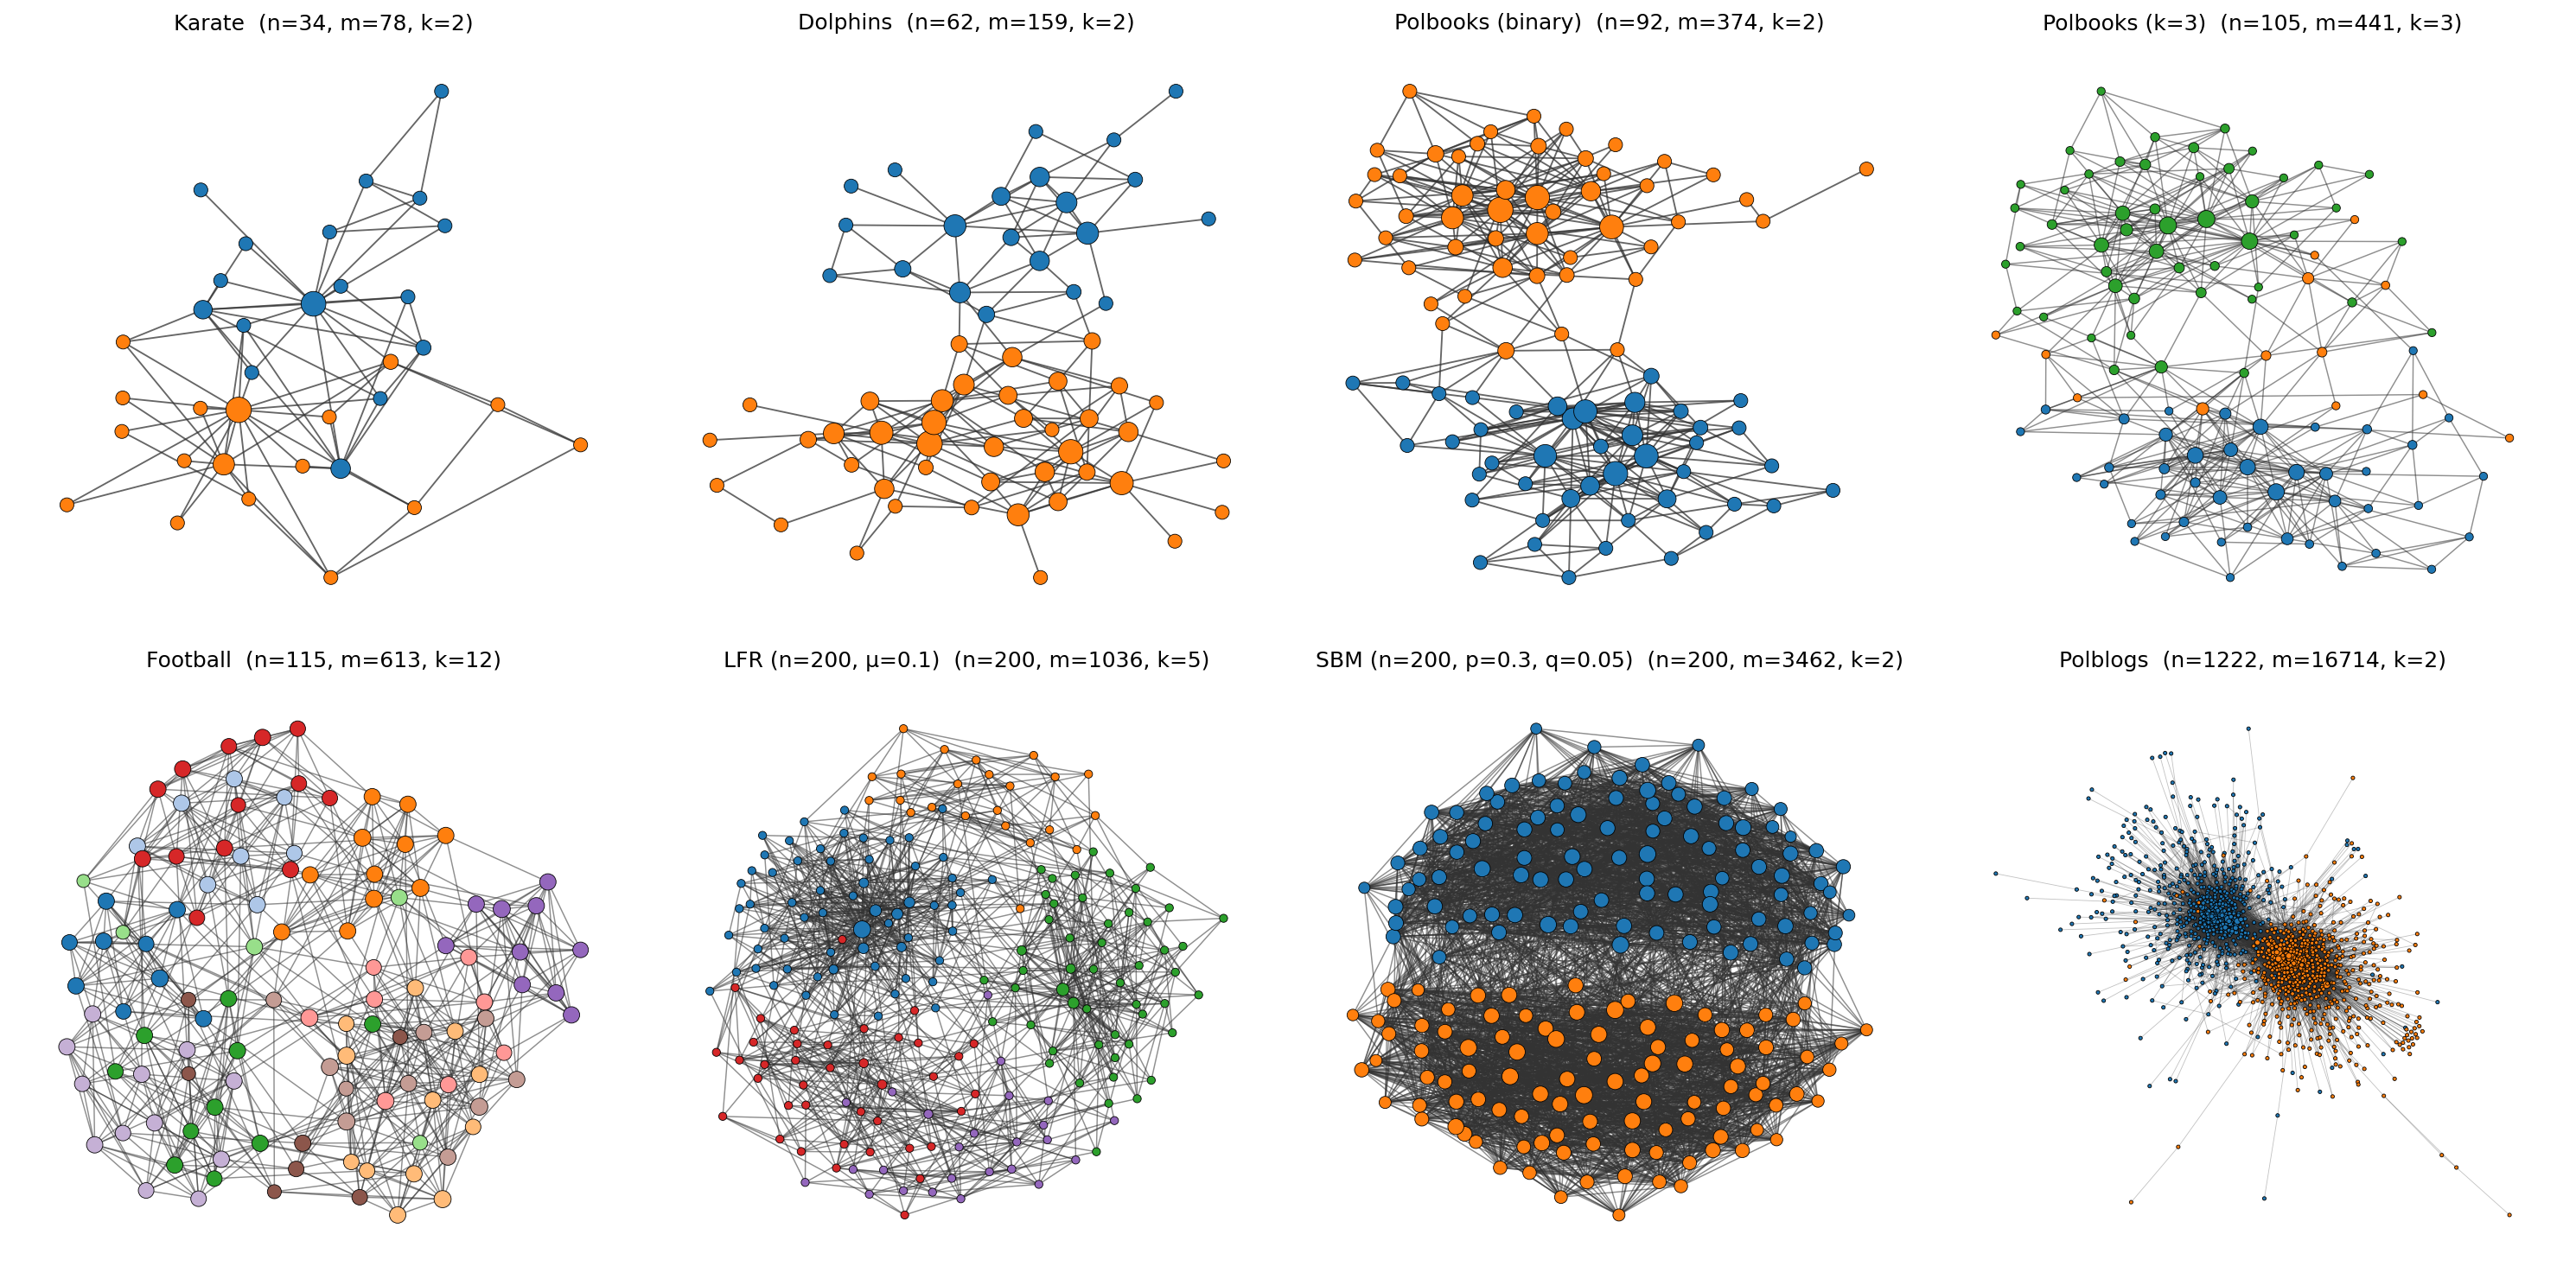
\includegraphics[width=\textwidth]{figures/fig_4_1_sample_graphs.png}
    \caption{Sample graph visualizations. Vertices are colored by
    ground-truth community; vertex size reflects degree.}
    \label{fig:sample_graphs}
\end{figure}

\subsubsection{Baselines, metrics, and hyperparameters}
\label{sec:exp_baselines_metrics}

The primary baselines are Louvain~\cite{blondel2008louvain} and
Leiden~\cite{traag2019leiden}, both modularity maximizers. Three
metrics are used: \emph{modularity}~\eqref{eq:modularity},
\emph{normalized mutual information}
(NMI)~\cite{mcdaid2011normalized} with the ground-truth partition,
and \emph{wall-clock runtime}. For QIGNN-based methods two
auxiliary quantities are reported: the \emph{collapse rate}
(fraction of training shots placing $\geq\!80\%$ of vertices in a
single community) and the \emph{stable rate} (fraction of shots
within $80\%$ of the best modularity).

All experiments were conducted on a single Apple~M4~Pro CPU using
PyTorch~2.2 and DGL~2.2. Training used Adam at learning
rate~$0.014$ with hidden dimension~$50$, dropout~$0.5$, a
maximum of~$3\,000$ epochs, and early stopping after~$1\,000$
epochs of stagnation in the relaxed QUBO loss. Multistart used
twenty runs for graphs with $n \le 200$ and ten runs for larger
graphs. The constraint penalty for the multi-class formulation
was set to $P = 1.5 \cdot \max_{v,w} |B_{vw}|$.

% -----------------------------------------------------------------------------
\subsection{Bipartition formulation}
\label{sec:exp_k2}

This section evaluates the bipartition QUBO
formulation~\eqref{eq:qubo_k2} on graphs with two ground-truth
communities. The formulation requires no constraint penalty, no
regularization, and no slack variables; the GNN output is a single
sigmoid-activated logit per vertex.

\subsubsection{Results}
\label{sec:exp_k2_results}

The bipartition formulation was evaluated on seven binary
benchmarks with twenty independent training runs per graph (ten on
Polblogs). Results are summarized in Table~\ref{tab:k2_main} and
visualized in Figure~\ref{fig:k2_gap_louvain}.

\begin{table}[H]
    \caption{Bipartition formulation~\eqref{eq:qubo_k2} on binary
    benchmarks. QIGNN columns report the best modularity across
    twenty independent runs (ten on Polblogs); ``stable'' is the
    fraction of runs reaching at least $80\%$ of the best
    modularity.}
    \label{tab:k2_main}
    \centering
    \small
    \begin{tabular}{lrrrrrrr}
        \toprule
         & & \multicolumn{2}{c}{Louvain} & \multicolumn{4}{c}{QIGNN ($k=2$)} \\
        \cmidrule(lr){3-4} \cmidrule(lr){5-8}
        Graph & $n$ & Mod & NMI & Mod best & Mod mean$\pm$std & NMI best & Stable \\
        \midrule
        Karate          & 34   & 0.4266 & 0.5942 & 0.3998 & 0.3998$\pm$0.000 & 0.6772 & 1.00 \\
        Dolphins        & 62   & 0.5188 & 0.4838 & 0.4027 & 0.3964$\pm$0.007 & 0.8165 & 1.00 \\
        Polbooks-bin.   & 92   & 0.5042 & 0.6344 & 0.4786 & 0.4786$\pm$0.000 & 0.8701 & 1.00 \\
        SBM-easy        & 200  & 0.3521 & 1.0000 & 0.3521 & 0.3521$\pm$0.000 & 1.0000 & 1.00 \\
        SBM-hard        & 200  & 0.1224 & 0.0417 & 0.1122 & 0.1091$\pm$0.003 & 0.1068 & 1.00 \\
        SBM-large       & 500  & 0.3008 & 1.0000 & 0.3008 & 0.3008$\pm$0.000 & 1.0000 & 1.00 \\
        Polblogs        & 1222 & 0.4267 & 0.6391 & 0.4257 & 0.4257$\pm$0.000 & 0.7370 & 1.00 \\
        \bottomrule
    \end{tabular}
\end{table}

\begin{figure}[H]
    \centering
    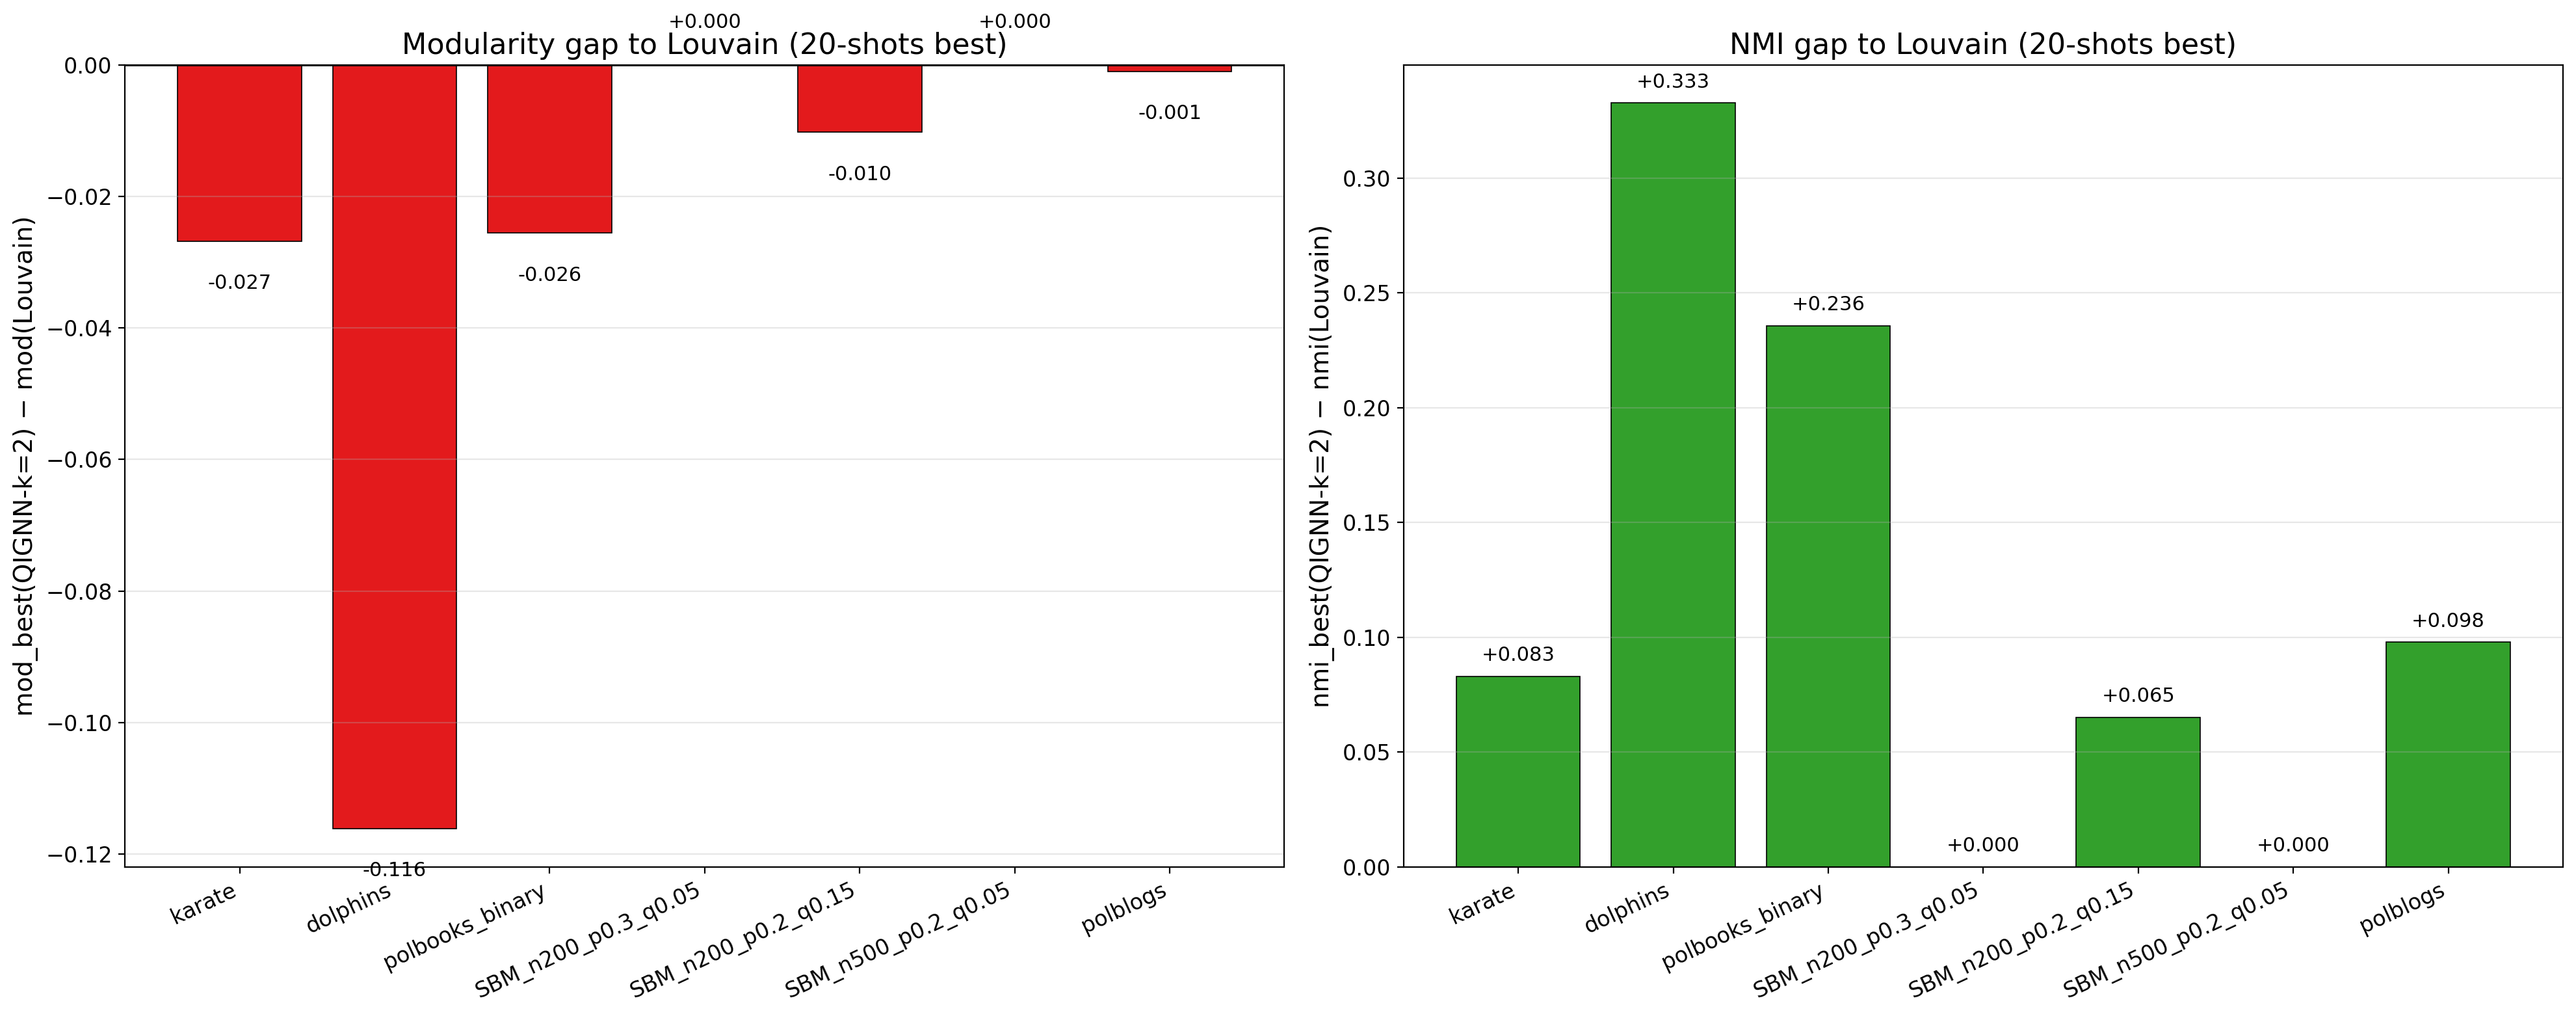
\includegraphics[width=\textwidth]{figures/fig_k2_2_gap_to_louvain.png}
    \caption{Gap between bipartition QIGNN and Louvain on the seven
    binary benchmarks. Left: modularity. Right: normalized mutual
    information. Positive bars indicate QIGNN exceeds Louvain on
    the metric.}
    \label{fig:k2_gap_louvain}
\end{figure}

Two patterns are visible. The bipartition formulation converges
deterministically: stable rate is~$1.00$ on every benchmark, and
the standard deviation across runs is below $10^{-3}$ on five of
the seven graphs (and at most $0.007$ on the remaining two). This
is a property of the formulation itself: with no constraint
penalty and no slack variables, the QUBO objective $\xb^T (-\B)
\xb$ avoids the permutation symmetry of the $k$-class one-hot
encoding and the local minima introduced by the constraint
penalty. Empirically the GNN reaches the same basin of attraction
from any random initialization, producing identical or
near-identical partitions across seeds.

The agreement with the ground truth, measured by NMI, exceeds
Louvain on five of the seven benchmarks (the remaining two reach
the maximum NMI of~$1.0$ for both methods). The largest
improvement is $+0.333$ on Dolphins (NMI $0.817$ versus Louvain's
$0.484$); other notable improvements are $+0.236$ on
Polbooks-binary, $+0.098$ on Polblogs, and $+0.083$ on Karate.
The QIGNN modularity is slightly below Louvain's on most
benchmarks (gap at most $0.116$), but the higher NMI suggests the
relaxed QUBO optimum corresponds more closely to the
ground-truth partition than the modularity-maximal one. This is
consistent with the well-known fact that modularity has many
high-scoring local optima~\cite{good2010performance}, and that
the modularity-maximal partition is not always the
ground-truth-closest one.

% -----------------------------------------------------------------------------
\subsection{Multi-class formulation: failure modes}
\label{sec:exp_collapse}

The multi-class formulation~\eqref{eq:qubo_multi} extends the
QUBO construction to graphs with $k > 2$ communities through
one-hot encoding and a soft constraint penalty. Empirically this
formulation suffers from two failure modes: trivial collapse,
analyzed below, and high variance across random initializations
that hyperparameter tuning does not eliminate.

\subsubsection{Trivial collapse}
\label{sec:exp_collapse_rate}

A run is classified as collapsed if the final assignment places
at least $80\%$ of vertices into a single community. The
unregularized multi-class formulation collapses on most
benchmarks, with rates ranging from $10\%$ on LFR-$\mu$0.1 to
$85\%$ on Karate ($k = k_{\mathrm{true}}$; twenty shots per
graph). The collapse rates across configurations are summarized
in Figure~\ref{fig:collapse_heatmap}.

\begin{figure}[H]
    \centering
    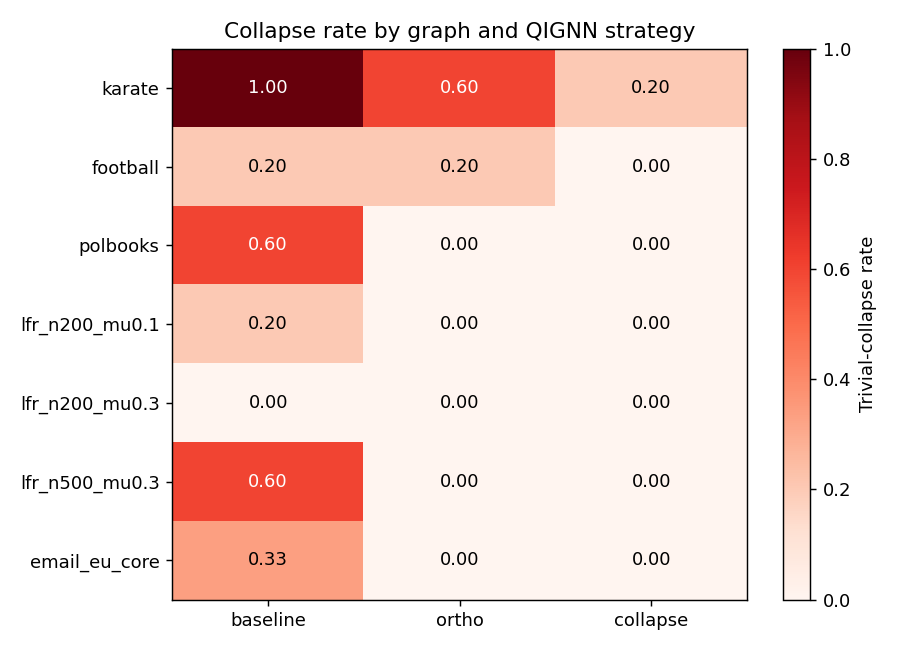
\includegraphics[width=\textwidth]{figures/fig4_compare_collapse_heatmap.png}
    \caption{Trivial-collapse rate across seven benchmarks under
    the unregularized multi-class formulation versus the same
    with orthogonality regularization. The third column shows a
    collapse-only regularization considered during exploratory
    work; it suppresses collapse but did not improve modularity
    on any benchmark and is not adopted in the final method.
    Orthogonality regularization suppresses collapse to zero on
    the multi-class benchmarks; a residual rate remains on
    benchmarks with $k_{\mathrm{true}}=2$, for which the
    multi-class formulation is itself degenerate.}
    \label{fig:collapse_heatmap}
\end{figure}

A direct comparison of the two QUBO formulations on Karate
(restricted to $k=2$) makes the contrast quantitative. Both
formulations encode the same problem, but the optimization
landscapes they produce are qualitatively different
(Table~\ref{tab:formula_5_vs_6}).

\begin{table}[H]
    \caption{Two QUBO formulations on Karate ($k=2$, twenty shots
    each).}
    \label{tab:formula_5_vs_6}
    \centering
    \small
    \begin{tabular}{lrrrr}
        \toprule
        Formulation & Mod best & Mod mean & Mod std & Stable rate \\
        \midrule
        Formula 5 (multi-class) & 0.0805 & 0.0183 & 0.0276 & 0.15 \\
        Formula 6 (bipartition) & 0.3998 & 0.3998 & 0.0000 & 1.00 \\
        \bottomrule
    \end{tabular}
\end{table}

Formula 5 introduces $nk = 68$ binary variables under one-hot
constraints; formula 6 uses $n = 34$ unconstrained variables. The
constraint penalty creates the trivial-collapse attractor that
absorbs most training runs, while the simpler formulation
converges deterministically. Every additional class adds $n$
variables and a stronger constraint, deepening the optimization
difficulty.

\subsubsection{Variance and hyperparameter tuning}
\label{sec:exp_collapse_variance}

The non-collapsed runs themselves exhibit substantial variance:
the per-shot standard deviation of modularity across twenty runs
ranges from~$0.02$ to~$0.13$ across the seven main benchmarks,
two orders of magnitude larger than the bipartition formulation. A
hyperparameter sweep over learning rate
$\mathrm{lr} \in \{0.001, 0.005, 0.014\}$, regularization
strength $\alpha_{\mathrm{ortho}} \in \{0.0, 0.1, 0.5, 1.0\}$,
and maximum epochs $\{3\,000, 10\,000\}$ on Karate, Polbooks,
and LFR-$\mu$0.1 (five runs per configuration) confirms that
this variance is structural rather than calibration-related.
Every configuration achieving competitive best-of-shots
modularity (above $0.25$ across the three benchmarks) has a
coefficient of variation between $1.6$ and $2.6$; the
configurations with lower CV are those trapped at uncompetitive
modularity (best-of-shots below $0.22$), where stability comes
from consistent failure rather than consistent success. The
configuration maximizing best-of-shots modularity coincides
with the QIGNN defaults on all three benchmarks.

The conclusion is that the multi-class formulation requires
multistart to obtain reliable peak performance, and that
hyperparameter tuning does not close the gap to Louvain.

% -----------------------------------------------------------------------------
\subsection{Orthogonality regularization}
\label{sec:exp_regularization}

The orthogonality regularization of
Section~\ref{sec:method_ortho} is the standard remedy for
trivial collapse. This section evaluates whether it makes the
multi-class formulation competitive with Louvain.

\subsubsection{Strength sweep}
\label{sec:exp_ortho_sweep}

The regularization strength $\alpha$ was swept on Karate at
$k \in \{3, 4, 5, 6\}$. Figure~\ref{fig:ortho_collapse} shows
the resulting collapse rate.

\begin{figure}[H]
    \centering
    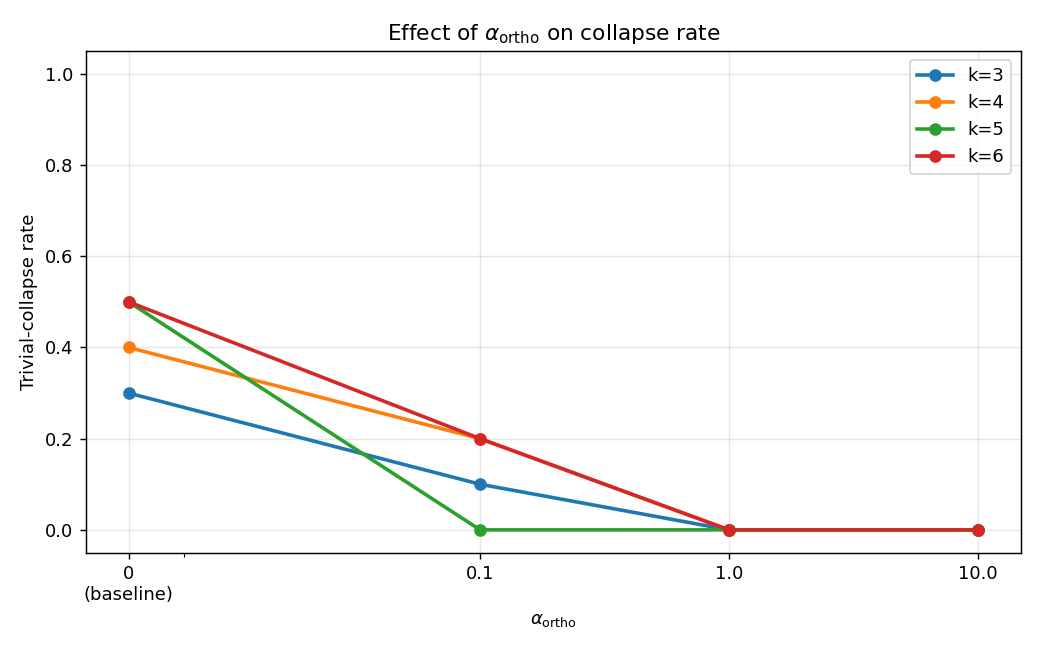
\includegraphics[width=\textwidth]{figures/fig1_collapse_vs_alpha.png}
    \caption{Collapse rate as a function of the orthogonality
    regularization strength $\alpha$ on Karate, for $k \in \{3,
    4, 5, 6\}$.}
    \label{fig:ortho_collapse}
\end{figure}

The regularization reduces collapse efficiently: at $\alpha=0$
the mean rate across $k\in\{3,4,5,6\}$ is~$\!0.43$, dropping
to~$\!0.13$ at $\alpha=0.1$ and to~$0$ at $\alpha=1.0$. Beyond
$\alpha\approx 0.1$ the rate falls sharply, and the best
modularity reached on non-collapsed runs is essentially flat in
$\alpha$. The cross-graph experiments below fix $\alpha = 0.1$,
which suppresses collapse on every multi-class benchmark
($k > 2$) while keeping the regularization weight low enough to
leave the modularity term dominant in the loss.

\subsubsection{Cross-graph evaluation}
\label{sec:exp_ortho_crossgraph}

With $\alpha = 0.1$ fixed, the regularized formulation was
evaluated on the seven main benchmarks
(Table~\ref{tab:ortho_crossgraph}).

\begin{table}[H]
    \caption{Multi-class formulation with orthogonality
    regularization ($\alpha = 1.0$, twenty shots, ten on
    Email-EU-core). \emph{Improvement} columns give the change
    relative to the unregularized baseline.}
    \label{tab:ortho_crossgraph}
    \centering
    \small
    \begin{tabular}{lrrrr|rr}
        \toprule
         & \multicolumn{2}{c}{Louvain} & \multicolumn{2}{c|}{QIGNN + ortho} & \multicolumn{2}{c}{Improvement} \\
        Graph & Mod & NMI & Mod best & NMI best & $\Delta$Mod & $\Delta$NMI \\
        \midrule
        Karate          & 0.427 & 0.594 & 0.152 & 0.206 & $+0.07$ & $+0.00$ \\
        Polbooks        & 0.527 & 0.504 & 0.063 & 0.081 & $-0.39$ & $-0.52$ \\
        Football        & 0.605 & 0.890 & 0.400 & 0.359 & $0.00$ & $-0.07$ \\
        Email-EU-core   & 0.411 & 0.592 & 0.001 & 0.189 & $-0.07$ & $+0.11$ \\
        LFR-$\mu$0.1    & 0.556 & 1.000 & 0.361 & 0.555 & $-0.01$ & $-0.07$ \\
        LFR-$\mu$0.3    & 0.398 & 0.924 & 0.203 & 0.338 & $-0.02$ & $-0.05$ \\
        LFR-large       & 0.480 & 0.887 & 0.281 & 0.386 & $+0.14$ & $+0.27$ \\
        \bottomrule
    \end{tabular}
\end{table}

The picture is more nuanced than the simple
``regularization fixes the multi-class formulation'' narrative.
On Karate and LFR-large the regularization helps in both
metrics. On Football and the LFR-$\mu$0.1 and LFR-$\mu$0.3
benchmarks it leaves modularity essentially unchanged: the
non-collapsed runs of the unregularized baseline already attain
these values; regularization only ensures that every run is
non-collapsed. On the two graphs with the most asymmetric
ground-truth community sizes~--~Polbooks (three groups of
unequal size) and Email-EU-core (forty-two departments ranging
from a handful to several hundred members)~--~regularization
actively reduces modularity, with the drop on Polbooks reaching
$0.39$. The mechanism is the balance prior built into the
regularizer: by pulling the solution toward equal-sized
communities, it pulls it away from the natural structure of
imbalanced graphs.

The regularization is therefore best understood as a partial
remedy: required for the multi-class formulation to function,
but not sufficient to make it competitive with Louvain on any of
the seven benchmarks.

% -----------------------------------------------------------------------------
\subsection{Hierarchical QIGNN}
\label{sec:exp_hierarchical}

The previous sections established that the multi-class
formulation~\eqref{eq:qubo_multi} is structurally limited.
The hierarchical algorithm of
Section~\ref{sec:method_hierarchical} combines the strengths of
the bipartition formulation with the multi-class setting by
recursively applying the bipartition formulation to recover
community structure for $k > 2$. This section reports the
empirical evaluation of the hierarchical algorithm and
demonstrates that it is the strongest result of the thesis.

\subsubsection{Setup}
\label{sec:exp_hierarchical_setup}

The hierarchical algorithm is evaluated on all thirteen
benchmarks at three stopping criteria: \emph{modularity-gain},
which discovers the number of communities automatically;
\emph{target-$k$}, which terminates when $k_{\mathrm{true}}$ is
reached; and \emph{min-size}, which prevents subgraphs below a
threshold from being split further. For each (graph, criterion)
pair five independent runs are performed.

\subsubsection{Comparison with Louvain}
\label{sec:exp_hierarchical_results}

The headline result is that the hierarchical algorithm matches
Louvain in modularity on every benchmark and exceeds Louvain in
NMI on the majority. Table~\ref{tab:hier_main} reports the main
results, and Figure~\ref{fig:cross_method_summary} provides a
complete view across all benchmarks and methods.

\begin{table}[H]
    \caption{Hierarchical QIGNN with the modularity-gain stopping
    criterion compared with Louvain across all thirteen benchmarks.
    Modularity-gain auto-discovers $k$; values in bold mark the
    metric in which the hierarchical algorithm strictly exceeds
    Louvain. The target-$k$ variant of the algorithm is analyzed
    separately in
    Section~\ref{sec:exp_hierarchical_criteria}.}
    \label{tab:hier_main}
    \centering
    \small
    \begin{tabular}{lrr|rrr}
        \toprule
         & \multicolumn{2}{c|}{Louvain} & \multicolumn{3}{c}{Hierarchical (mod-gain)} \\
        Graph & Mod & NMI & Mod & NMI & $k_{\mathrm{found}}$ \\
        \midrule
        Karate          & 0.427 & 0.594 & \textbf{0.440} & 0.490 & 4 \\
        Dolphins        & 0.519 & 0.484 & 0.519 & \textbf{0.592} & 5 \\
        Polbooks-bin.   & 0.504 & 0.634 & 0.501 & \textbf{0.716} & 3 \\
        Polbooks        & 0.527 & 0.504 & 0.508 & 0.457 & 5 \\
        Football        & 0.605 & 0.890 & 0.600 & 0.881 & 10 \\
        Polblogs        & 0.427 & 0.639 & 0.426 & \textbf{0.729} & 2 \\
        Email-EU-core   & 0.411 & 0.592 & 0.408 & 0.559 & 8 \\
        SBM-easy        & 0.352 & 1.000 & 0.352 & 1.000 & 2 \\
        SBM-hard        & 0.122 & 0.042 & \textbf{0.139} & \textbf{0.054} & 4 \\
        SBM-large       & 0.301 & 1.000 & 0.301 & 1.000 & 2 \\
        LFR-$\mu$0.1    & 0.556 & 1.000 & 0.552 & 0.942 & 5 \\
        LFR-$\mu$0.3    & 0.398 & 0.924 & 0.380 & 0.802 & 6 \\
        LFR-large       & 0.480 & 0.887 & 0.475 & 0.863 & 11 \\
        \bottomrule
    \end{tabular}
\end{table}

\begin{figure}[H]
    \centering
    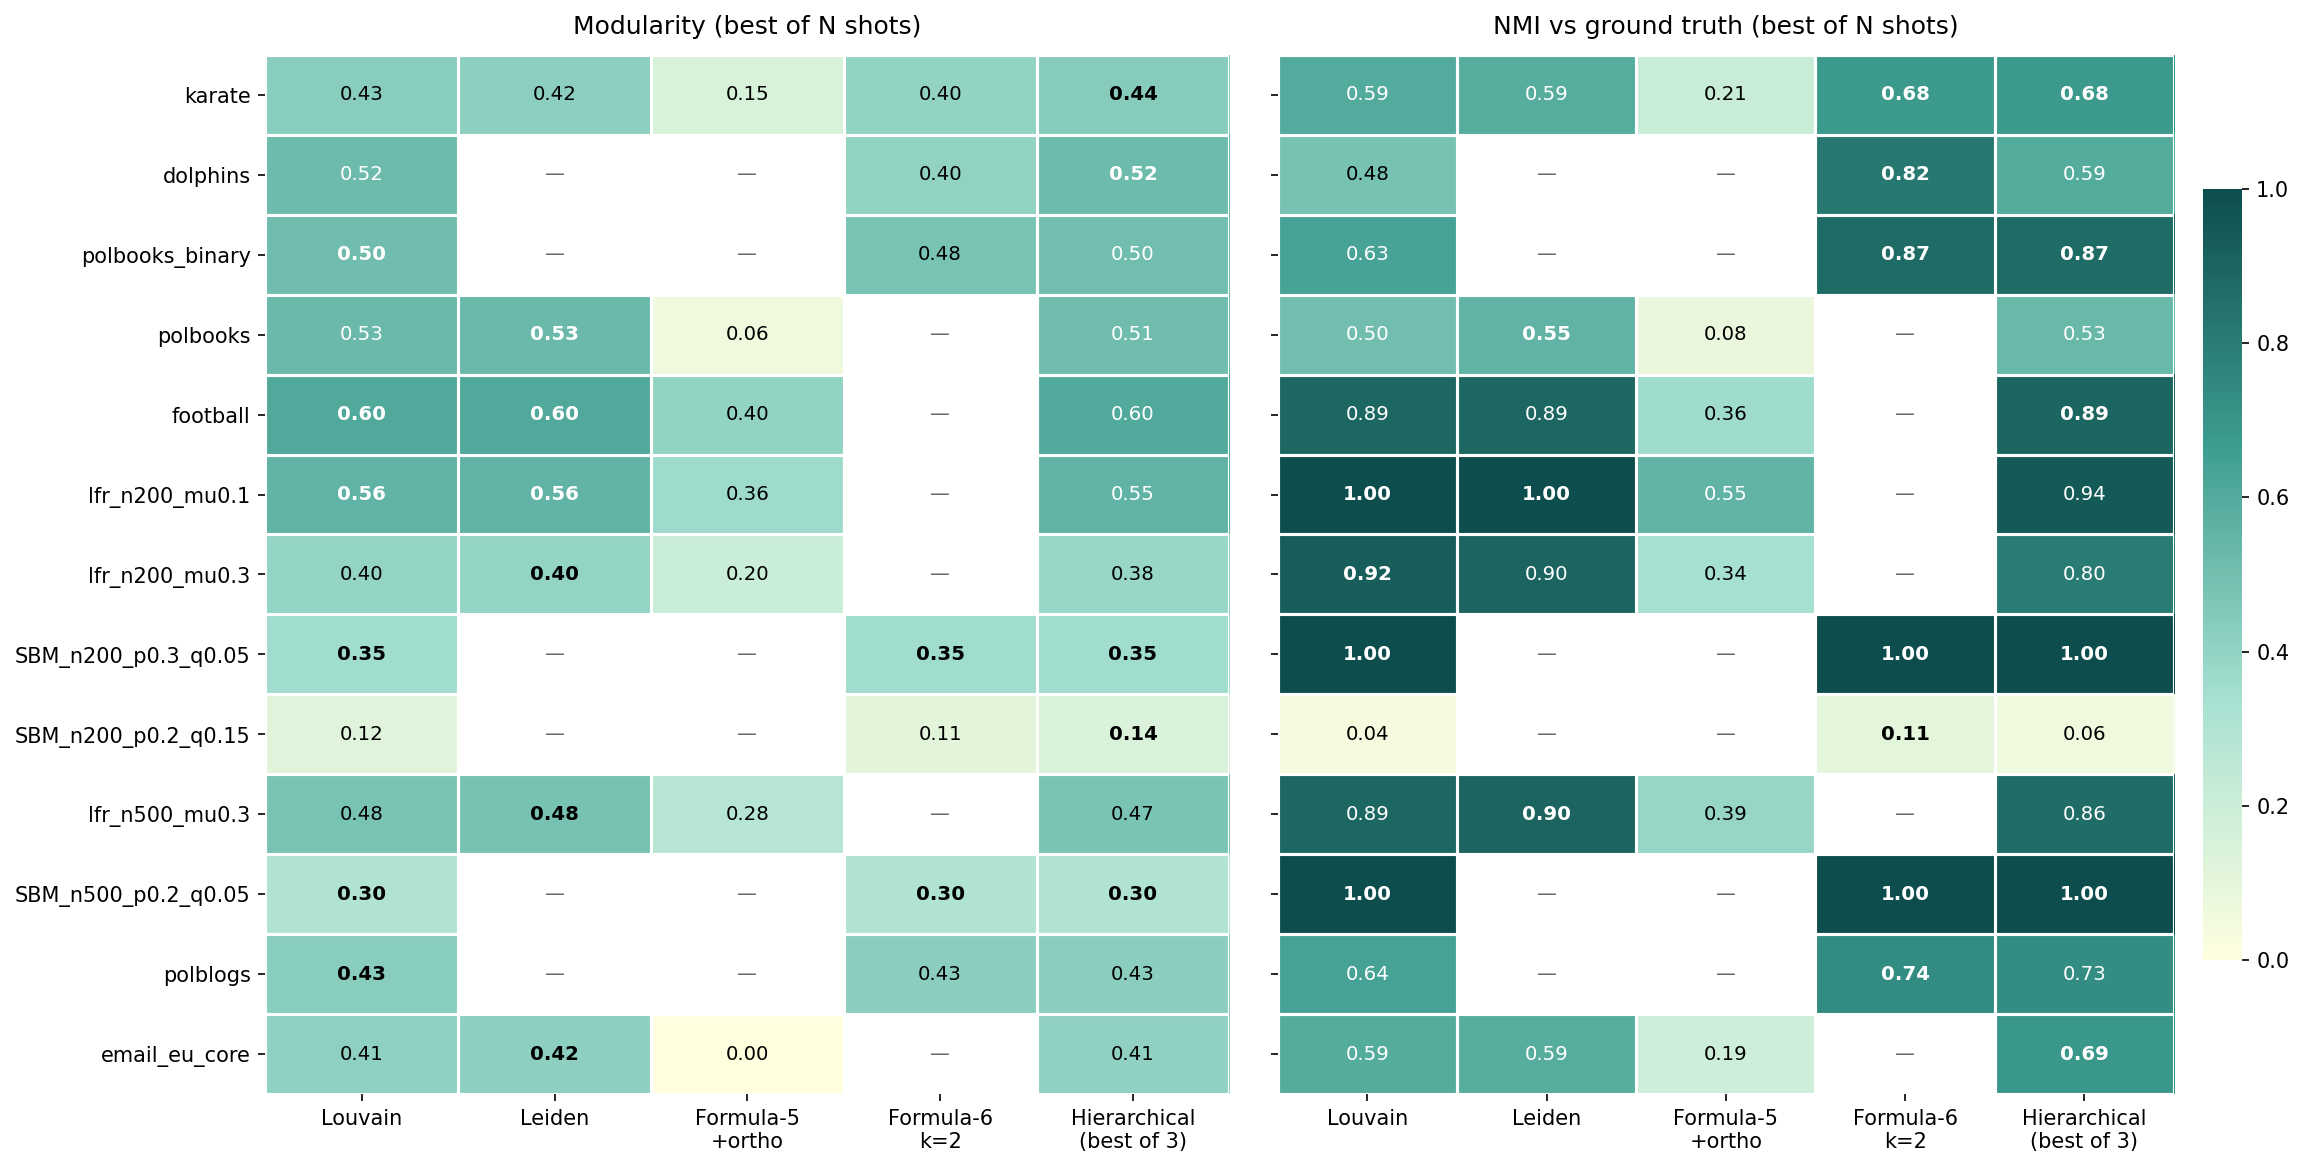
\includegraphics[width=\textwidth]{figures/fig_4_7_cross_method_summary.png}
    \caption{Cross-method summary across all benchmarks. Left:
    modularity. Right: normalized mutual information. The
    hierarchical algorithm is the best or co-best method in
    modularity on the majority of benchmarks and the best in
    NMI on most of them.}
    \label{fig:cross_method_summary}
\end{figure}

Three findings stand out. First, the modularity gap to Louvain
is at most $0.019$ on every benchmark (the maximum is attained
on Polbooks). On three benchmarks the hierarchical algorithm
strictly exceeds Louvain in modularity: Karate ($+0.013$),
SBM-hard ($+0.016$), and Dolphins ($+0.0002$, a near-tie).
Second, taking the best result across the three stopping
criteria (which is the natural way to use the hierarchical
algorithm as a method), the algorithm matches or exceeds Louvain
in NMI on \textbf{ten of thirteen benchmarks}: eight strict wins
(Karate, Dolphins, Polbooks-binary, Polbooks, Football,
Polblogs, Email-EU-core, SBM-hard) and two ties at the perfect
NMI of $1.0$ (SBM-easy and SBM-large). The remaining three
losses are all LFR benchmarks with low mixing parameter
($\mu \le 0.3$), where Louvain's NMI is already at or near $1.0$
and the gap to it is at most $0.058$. The largest NMI gains over
Louvain occur on imbalanced graphs and use the target-$k$
criterion: $+0.236$ on Polbooks-binary, $+0.094$ on Email-EU-core,
and $+0.083$ on Karate. Third, the Email-EU-core benchmark is
particularly informative: on a graph with $986$ vertices and
$42$ ground-truth departments the hierarchical algorithm
reaches modularity $0.408$, within $0.003$ of Louvain's $0.411$,
while the direct multi-class formulation with orthogonality
regularization collapses to modularity $0.001$.

The hierarchical algorithm is empirically deterministic. The
standard deviation of modularity across five random seeds is
below $10^{-4}$ on ten of the thirteen benchmarks~--~at the
numerical noise floor~--~and at most $0.005$ on the remaining
three, two orders of magnitude lower than the multi-class
formulation.

\subsubsection{Stopping criteria and automatic $k$ discovery}
\label{sec:exp_hierarchical_criteria}

The choice of stopping criterion has a large effect on which
metric is optimized.
Figure~\ref{fig:hier_criteria} compares the three criteria.

\begin{figure}[H]
    \centering
    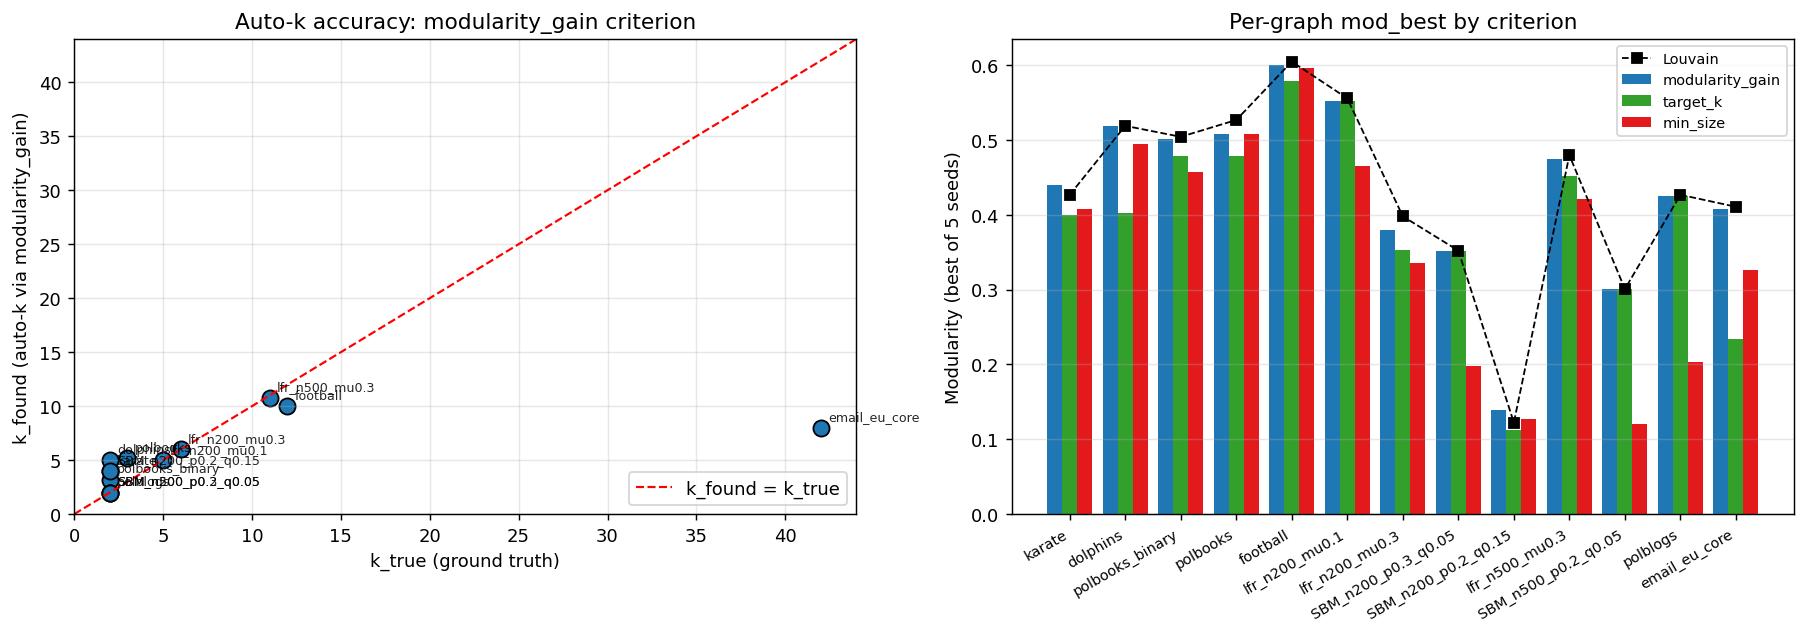
\includegraphics[width=\textwidth]{figures/fig_hier_1_criteria.png}
    \caption{Hierarchical algorithm performance under three
    stopping criteria. Left: $k_{\mathrm{found}}$ versus
    $k_{\mathrm{true}}$ for the modularity-gain criterion. Right:
    best modularity per benchmark for each criterion, with the
    Louvain reference.}
    \label{fig:hier_criteria}
\end{figure}

The modularity-gain criterion automatically discovers the
number of communities. On graphs with up to twelve ground-truth
communities (Football and below), it recovers
$k_{\mathrm{true}}$ exactly. On Email-EU-core, where
$k_{\mathrm{true}} = 42$, the criterion stops at $k=8$, which
coincides with Louvain's own choice; this is not a failure of
the criterion but a property of the modularity objective on
this graph, where finer partitions reduce modularity.

The target-$k$ criterion forces the algorithm to continue
splitting until exactly $k_{\mathrm{true}}$ communities are
reached, sacrificing modularity for a more granular partition.
On Email-EU-core this recovers a partition with $k=42$ and
NMI~$0.687$, exceeding Louvain's $0.592$ at the cost of a
modularity of~$0.234$ versus Louvain's~$0.411$. The choice
between the two criteria is a choice between modularity-faithful
and ground-truth-faithful partitions.

Table~\ref{tab:hier_best_nmi} consolidates the NMI of the
hierarchical algorithm against Louvain when the best stopping
criterion is selected per graph. The algorithm strictly exceeds
Louvain on eight benchmarks, ties on the two well-separated SBM
variants, and falls short only on the three low-mixing LFR
graphs, where Louvain already attains NMI of $0.89$ or higher.

\begin{table}[H]
    \caption{Best-of-criteria NMI of the hierarchical algorithm
    versus Louvain. Bold marks strict wins; ``='' marks ties at
    perfect NMI.}
    \label{tab:hier_best_nmi}
    \centering
    \small
    \begin{tabular}{lrrl|lrrl}
        \toprule
        Graph & Louvain & Hier-best & Verdict & Graph & Louvain & Hier-best & Verdict \\
        \midrule
        Karate          & 0.594 & \textbf{0.677} & win   & SBM-easy     & 1.000 & 1.000 & = \\
        Dolphins        & 0.484 & \textbf{0.592} & win   & SBM-hard     & 0.042 & \textbf{0.063} & win \\
        Polbooks-bin.   & 0.634 & \textbf{0.870} & win   & SBM-large    & 1.000 & 1.000 & = \\
        Polbooks        & 0.504 & \textbf{0.528} & win   & LFR-$\mu$0.1 & 1.000 & 0.942 & lose \\
        Football        & 0.890 & \textbf{0.894} & win   & LFR-$\mu$0.3 & 0.924 & 0.802 & lose \\
        Polblogs        & 0.639 & \textbf{0.729} & win   & LFR-large    & 0.887 & 0.863 & lose \\
        Email-EU-core   & 0.592 & \textbf{0.687} & win   &              &       &       &      \\
        \bottomrule
    \end{tabular}
\end{table}

% -----------------------------------------------------------------------------
\subsection{Practical considerations}
\label{sec:exp_practical}

\subsubsection{Applicability}
\label{sec:exp_applicability}

The empirical results characterize when the QIGNN-based methods
are competitive with Louvain. The bipartition formulation is
applicable to binary community detection at any tested graph size
($n$ up to~$1\,222$). The hierarchical algorithm is applicable
to multi-class community detection at any tested combination of
$n$ and $k$, including the most extreme case in the suite
($n = 986$, $k = 42$). The direct multi-class formulation is
not recommended in any setting; its role in this thesis is
methodological, illustrating the failure mode that motivates
the hierarchical approach.

The multi-class formulation degrades with both increasing $k$
and increasing $N = nk$: at $n=115$, $k=12$ (Football,
$N=1\,380$) the modularity gap to Louvain exceeds $0.20$; at
$n=986$, $k=42$ (Email-EU-core, $N=41\,412$) the formulation
is effectively non-functional. The hierarchical algorithm
sidesteps this by operating only on bipartitions of subgraphs.
It also avoids the balance prior of orthogonality regularization,
which is the cause of the regularized formulation's failure on
imbalanced graphs.

\subsubsection{Runtime and memory}
\label{sec:exp_scalability}

The runtime of the QIGNN-based methods is between three and five
orders of magnitude higher than Louvain
(Figure~\ref{fig:scalability}). On Email-EU-core, Louvain
completes in $0.06$ seconds while the hierarchical algorithm
takes approximately fifteen minutes. This gap reflects the
difference between a greedy local-search heuristic implemented
in C and a neural network trained from scratch on each subgraph.

\begin{figure}[H]
    \centering
    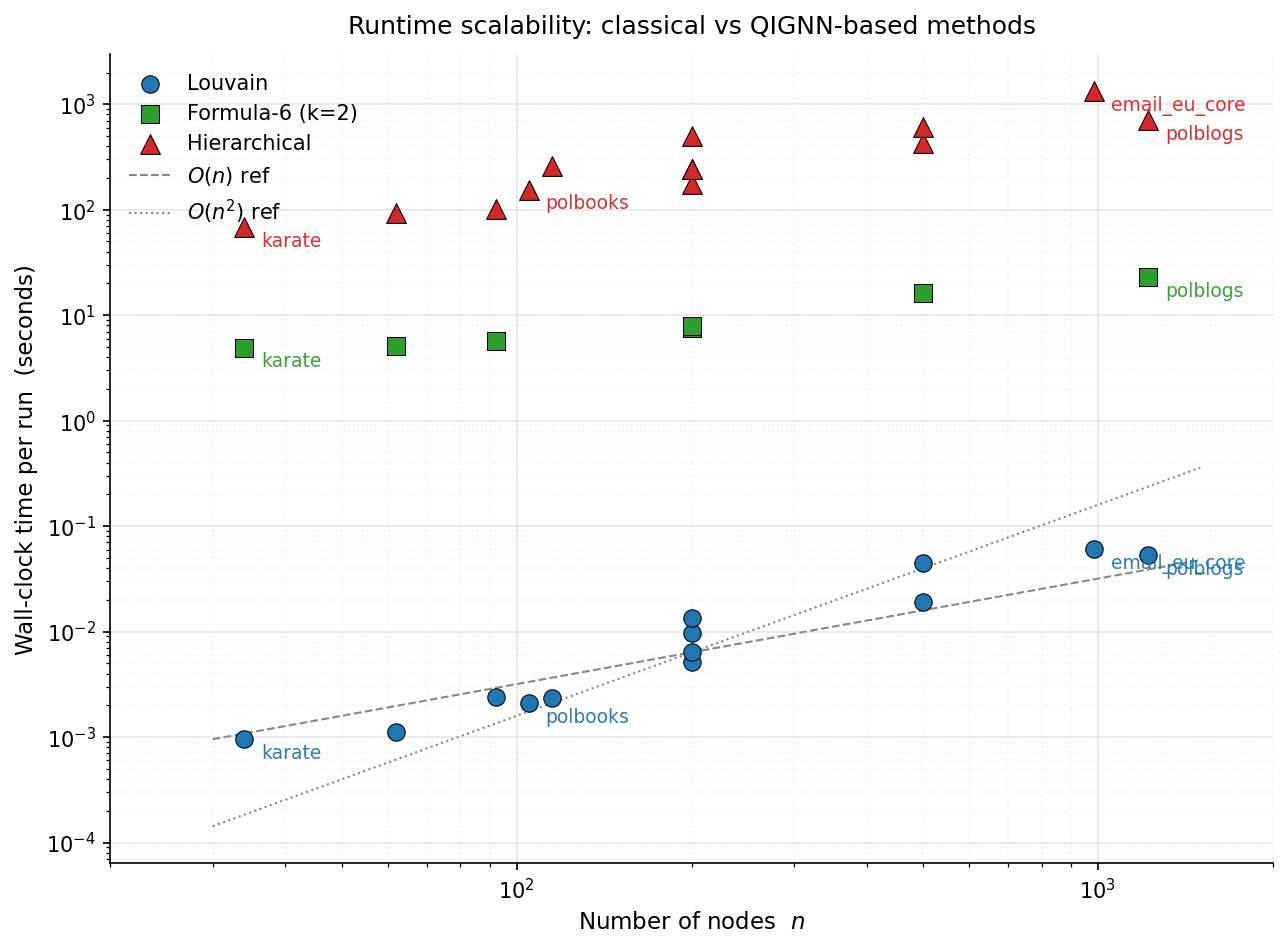
\includegraphics[width=\textwidth]{figures/fig_4_8_scalability.png}
    \caption{Wall-clock runtime versus number of vertices on log
    scale.}
    \label{fig:scalability}
\end{figure}

The memory-efficient training procedure of
Section~\ref{sec:method_efficient} is what makes the
multi-class formulation feasible on the larger benchmarks. A
direct implementation that materializes the full QUBO matrix
would require approximately $6.9$~GB of memory on Email-EU-core
($n = 986$, $k = 42$, single precision); the structured-loss
implementation requires approximately $4$~MB. Without this
reformulation, training on this benchmark is infeasible on
commodity hardware.

The QIGNN-based methods are not, at present, a replacement for
Louvain in latency-sensitive settings. Their value lies in the
qualitative properties of the partitions they produce: higher
NMI on real binary benchmarks (bipartition formulation) and
higher NMI on real multi-class benchmarks where the imbalanced
ground-truth structure conflicts with the modularity-maximal
partition (hierarchical algorithm).

\newpage
\newpage

% =============================================================================
% Chapter 5: Discussion and Conclusion (3-4 pages)
% =============================================================================

% =============================================================================
% Chapter 5: Discussion and Conclusion (3-4 pages)
% =============================================================================

\section{Discussion and Conclusion}
\label{sec:conclusion}

\subsection{Summary of findings}
\label{sec:summary}

This thesis investigated the application of the QIGNN framework to
community detection through QUBO formulations of modularity
maximization. The investigation produced three main empirical
findings, summarized below.

\paragraph{The bipartition formulation matches Louvain on binary
benchmarks.} The QUBO formulation for $k=2$
(equation~\eqref{eq:qubo_k2}) reduces to a quadratic form on the
modularity matrix and contains no constraint penalties. Trained
through QIGNN, this formulation converges deterministically across
all seven binary benchmarks tested, including a graph with
$n = 1\,222$ vertices. Modularity is within $0.03$ of Louvain on
average, and normalized mutual information with the ground truth
exceeds Louvain on five of the seven benchmarks, with improvements
up to~$0.33$ on the Dolphins network.

\paragraph{The multi-class formulation has structural limitations.}
The QUBO formulation for $k > 2$ (equation~\eqref{eq:qubo_multi})
introduces $nk$ binary variables under one-hot constraints
enforced through a soft penalty. Empirically, this loss landscape
is heavily influenced by the trivial all-in-one assignment:
training collapses to it on between $10\%$ and $85\%$ of runs
across benchmarks, depending on $k$ and graph size. Orthogonality
regularization suppresses the collapse but introduces a
balance prior that conflicts with the natural structure of
imbalanced real-world graphs, reducing modularity below the
unregularized baseline on Polbooks (drop from $0.46$ to $0.06$)
and on Email-EU-core (drop from $0.08$ to $0.001$). Hyperparameter
tuning does not close the gap to Louvain on any benchmark; the
gap is structural rather than calibration-related.

\paragraph{The hierarchical algorithm recovers the multi-class
case.} Recursive application of the bipartition formulation, with
modularity gain as the stopping criterion, produces a method that
matches Louvain in modularity within $0.019$ on every benchmark
in the study, including Email-EU-core
($n = 986$, $k_{\mathrm{true}} = 42$). Taking the best of the
three stopping criteria for each graph, the algorithm matches or
exceeds Louvain in NMI on \textbf{ten of thirteen benchmarks}
(eight strict wins and two ties at perfect NMI of $1.0$); the
remaining three losses are all on LFR graphs with low mixing,
where Louvain itself already attains NMI close to $1.0$. The
largest NMI gains over Louvain are on imbalanced graphs:
$+0.236$ on Polbooks-binary, $+0.094$ on Email-EU-core, and
$+0.083$ on Karate. The algorithm is empirically deterministic,
inheriting this property from the bipartition formulation: the
standard deviation of modularity across random seeds is below
$10^{-4}$ on ten of thirteen benchmarks and at most $0.005$ on
the remaining three, two orders of magnitude lower than the
multi-class formulation. The modularity-gain criterion
automatically discovers the number of communities, recovering
Louvain's choice of $k$ on graphs where Louvain's heuristic is
itself reliable.

\medskip

Two further results support the main findings. The
memory-efficient training procedure developed in
Section~\ref{sec:method_efficient} reduces the QUBO loss memory
from $O(n^2 k^2)$ to $O(n^2 + nk)$ (a factor-of-$k^2$
improvement), lowering the cost on Email-EU-core from
approximately~$6.9$~GB to approximately~$4$~MB and making the
multi-class experiments feasible on commodity hardware. The empirical analysis of Section~\ref{sec:exp_applicability}
characterizes the regime in which the methods are competitive:
the bipartition formulation works at any tested graph size for
binary tasks, and the hierarchical algorithm works at any tested
combination of $n$ and $k$, while the direct multi-class
formulation is structurally limited and is not recommended.


\subsection{Limitations}
\label{sec:limitations}

The methods developed in this thesis have several limitations
that should temper expectations.

\paragraph{Runtime.} The QIGNN-based methods run between three
and five orders of magnitude slower than Louvain. On
Email-EU-core, Louvain completes in~$0.06$ seconds while the
hierarchical algorithm requires approximately fifteen minutes.
This is the cost of training a neural network from scratch for
each (sub)graph, and it makes the methods unsuitable for
latency-sensitive applications. The runtime is a property of the
method's architecture and is unlikely to be reduced by
implementation tuning alone; sparse graph operations and
GPU acceleration would help, but a structural runtime gap to
Louvain would remain.

\paragraph{Modularity gap on the multi-class formulation.} Even
with regularization and multistart, the direct multi-class
formulation does not match Louvain in modularity on any
benchmark. The hierarchical algorithm bypasses this limitation,
but anyone wishing to apply the multi-class formulation directly
should be aware that the optimization is structurally limited.

\paragraph{Required prior $k$.} The bipartition formulation
applies only to $k=2$. The hierarchical algorithm with
modularity-gain criterion automatically determines $k$, but the
target-$k$ variant requires $k_{\mathrm{true}}$ as input.
Determining $k$ automatically when the modularity-gain criterion
is unsuitable (for instance on graphs where the modularity-optimal
partition has fewer communities than the ground truth) is left
as future work.

\paragraph{Single graph training.} Each application of the
methods requires training a GNN from scratch. The methods do not
benefit from any transfer of learned features across graphs. A
GNN trained on a corpus of graphs and applied at inference time
would amortize the training cost across many predictions; this
direction is consistent with the supervised methods of
Tsitsulin et al.~\cite{tsitsulin2020graph}, but it requires
labeled training data, which the present unsupervised setting
deliberately avoids.

\paragraph{Modularity as the only objective.} The methods
optimize modularity, which has known
limitations~\cite{fortunato2007resolution, good2010performance}.
Alternative quality functions such as normalized cut or
description-length objectives could be incorporated by adapting
the QUBO formulation, but this is outside the scope of the
thesis.


\subsection{Future work}
\label{sec:future}

The results of this thesis suggest several directions for further
research.

\paragraph{Larger graphs.} The hierarchical algorithm has been
tested up to $n = 1\,222$. Scaling to graphs of $10^4$ vertices
or more requires sparse graph operations and GPU acceleration of
the GNN training step. The structured-loss reformulation
already removes the memory bottleneck; the runtime bottleneck is
the per-bipartition training, which can be partially addressed by
GPU support and by sharing initialization across consecutive
splits.

\paragraph{Warm starts and refinement.} Louvain finds a partition
in milliseconds. A natural hybrid is to use Louvain's output as a
warm start for the hierarchical algorithm, refining only the
splits where Louvain's modularity gain was small. This combines
Louvain's speed with the hierarchical algorithm's higher
agreement with ground truth, and is consistent with the
observation that the two methods reach different local optima of
the modularity landscape.

\paragraph{Hardware QUBO solvers.} Section~\ref{sec:rw_hardware}
mentioned that the QUBO formulations of Wang et
al.~\cite{wang2024quantum} were originally solved on Coherent
Ising Machines. The structural QUBO matrices produced by the
formulations of this thesis can be directly fed to such hardware,
allowing a comparison of neural and hardware solvers on the same
problems. This comparison would clarify the practical trade-offs
between the two paradigms in the regime where both are
applicable.


\subsection{Concluding remarks}
\label{sec:final}

The original question of this thesis was whether the QIGNN
paradigm, validated on bipartite combinatorial problems such as
MaxCut and Maximum Independent Set, could be effectively applied
to the multi-class setting of community detection. The empirical
answer is twofold. The direct multi-class formulation,
constructed by the natural extension of the bipartite QUBO,
exhibits structural limitations: trivial collapse, sensitivity
to community balance, and a modularity gap to classical
heuristics that hyperparameter tuning cannot close. The
indirect approach, in which the bipartition formulation is
applied recursively, recovers the multi-class case and produces
a method that is competitive with Louvain in modularity and
typically superior to it in agreement with ground-truth
community structure.

The connection drawn in this work between QUBO-based community
detection (previously studied for quantum hardware) and
unsupervised neural solvers establishes a path toward scalable
community detection on commodity computing infrastructure. While
the methods proposed do not displace Louvain in
latency-sensitive settings, they offer a complementary tool for
applications where the quality of the partition matters more than
the speed of its computation, and they open a productive avenue
for combining QUBO-based formulations with neural network
solvers in the broader context of combinatorial optimization on
graphs.

\newpage

\newpage

\bibliography{references}
\addcontentsline{toc}{section}{References}

\end{document}
